%!TEX root = thesis.tex
\chapter{Results and Discussion}
\label{ch:results}

%Optimum angles and their corresponding electricity use were found for the building energy simulation for all hours of the year. For the radiation and PV evaluations, a grid-convergence study was performed and results of an optimizing angle strategy was compared to sun-tracking. The combined simulations could then be evaluated to find the most efficient overall combinations and the sensitivities of various parameters on the system performance was found.

%\section{Combined Evaluation}

By combining results for building energy simulations and PV electricity production, the overall optimum configurations can be found. Figures \ref{fig:monthly_altitude} and \ref{fig:monthly_azimuth} detail carpet-plots of the facade optimised to maximise PV generation, and minimise heating, cooling and lighting demands independently. The simulation was done for a total of 49 angle combinations with seven different states for the altitude and the azimuth angles, i.e. a step size of $15\degree$. While the altitude angles are shown in figure \ref{fig:monthly_altitude}, the coresponding azimuth angles of the same optimization are shown in figure \ref{fig:monthly_azimuth}.

\begin{figure*}
	\begin{center}
	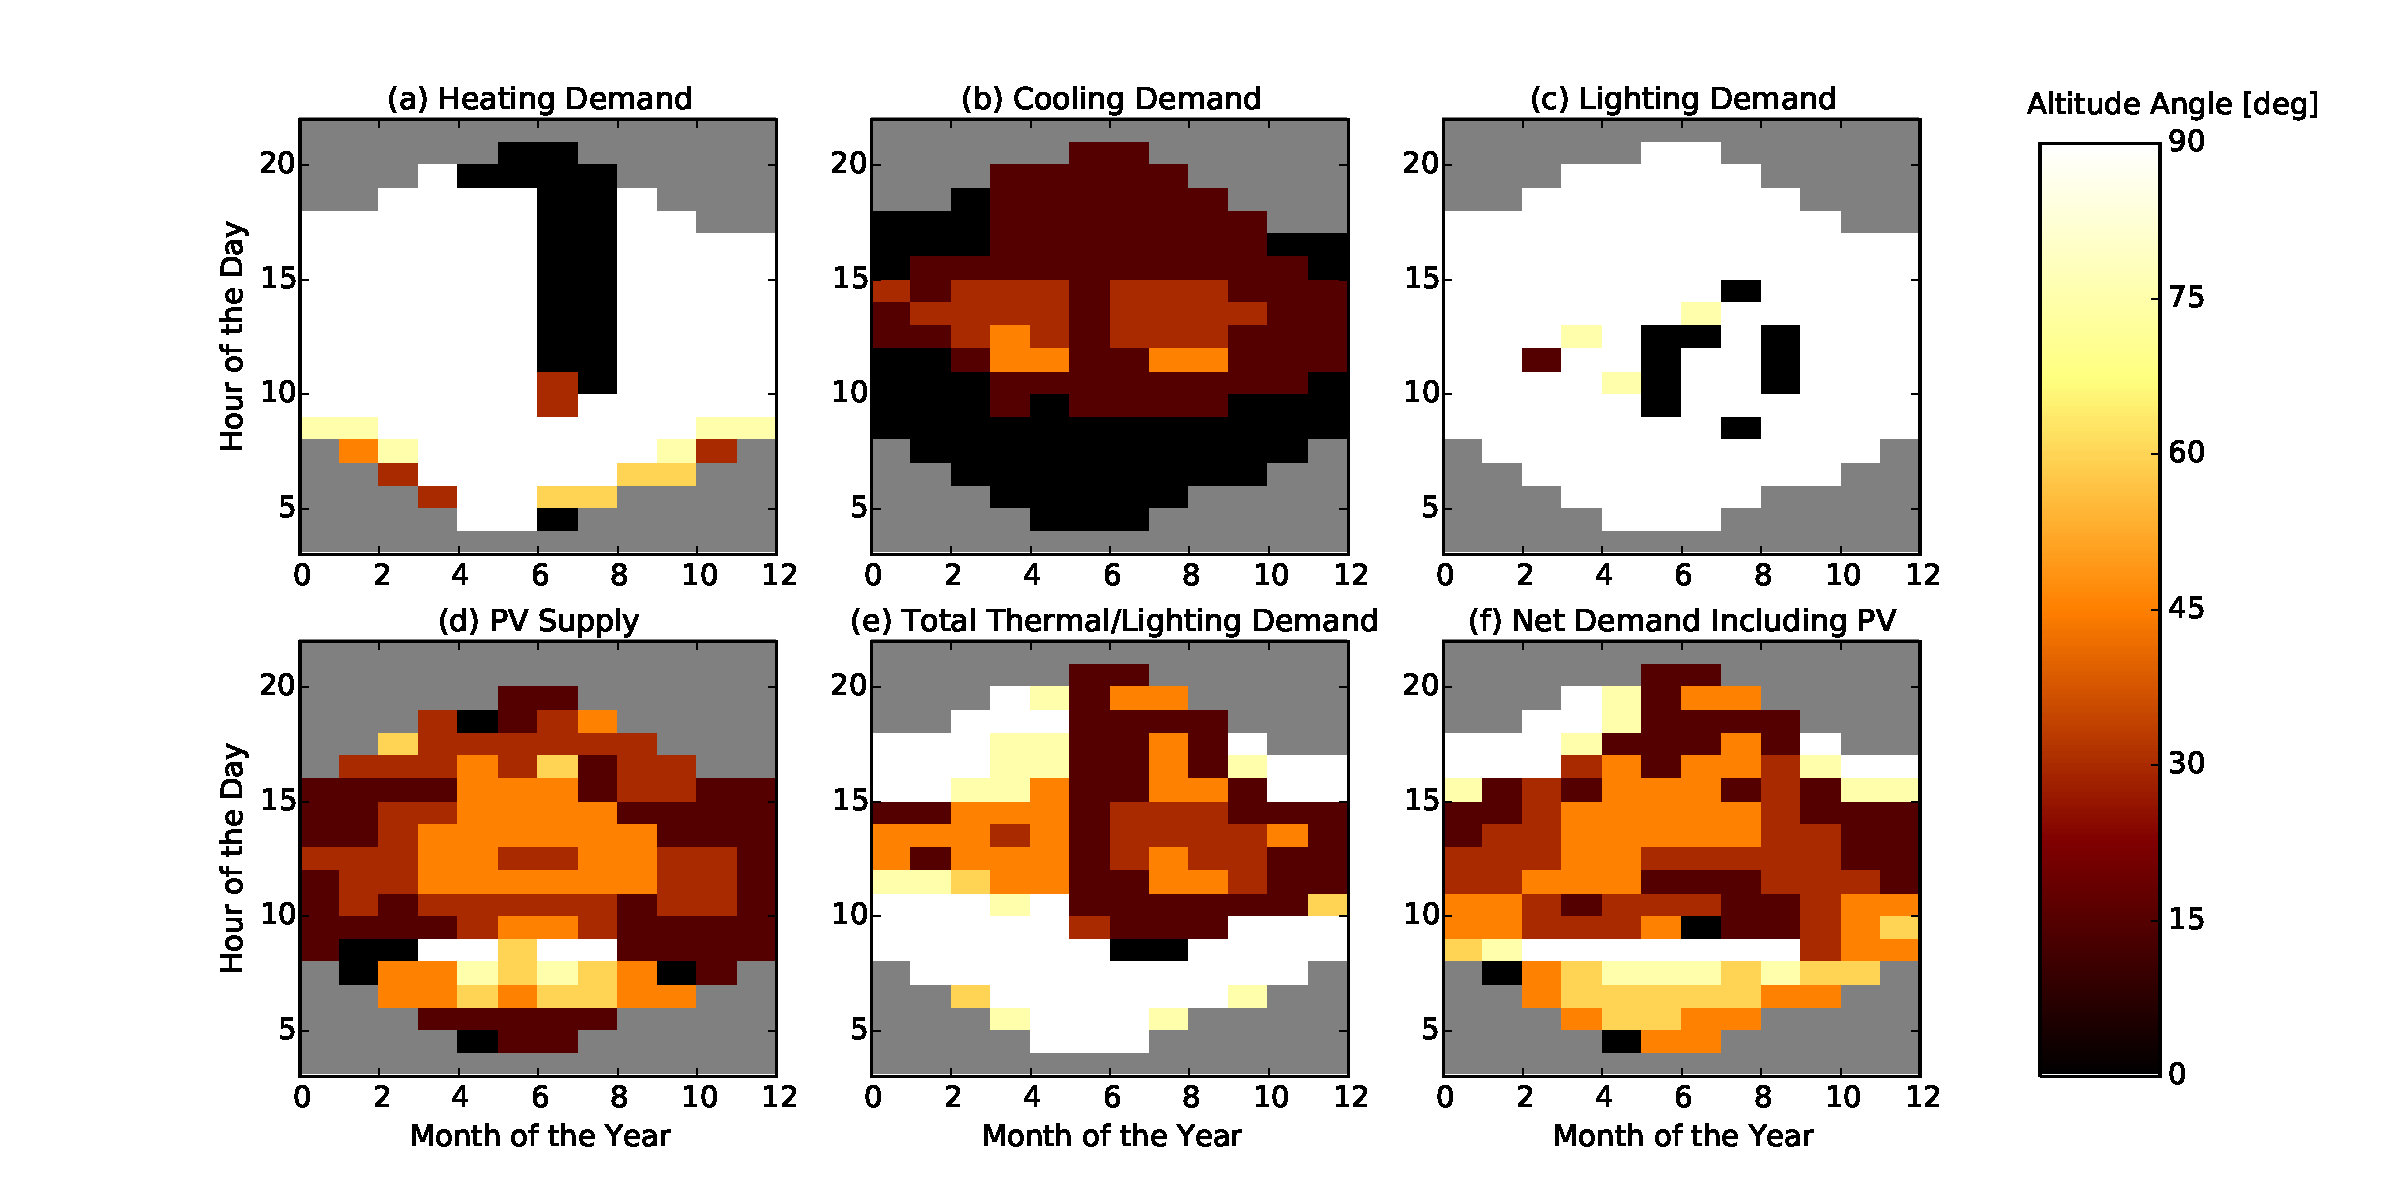
\includegraphics[width=\textwidth, trim= 1cm 0.5cm 1cm 1.4cm,clip]{monthly_altitude}
	\caption{Carpet plots detailing the optimal altitude angles to minimise the (a) heating demand, (b) cooling demand, (c) lighting demand, and (d) maximise PV electricity production. Figure (e) details the combinations for optimum building thermal management without PV production, (f) also includes the PV production. Small angles correspond to closed positions, whereas large angles represent open positions. The corresponding azimuth angles for each hour can be seen in the following figure (\ref{fig:monthly_azimuth}).}
	\label{fig:monthly_altitude}
	\end{center}
\end{figure*}

\begin{figure*}
	\begin{center}
	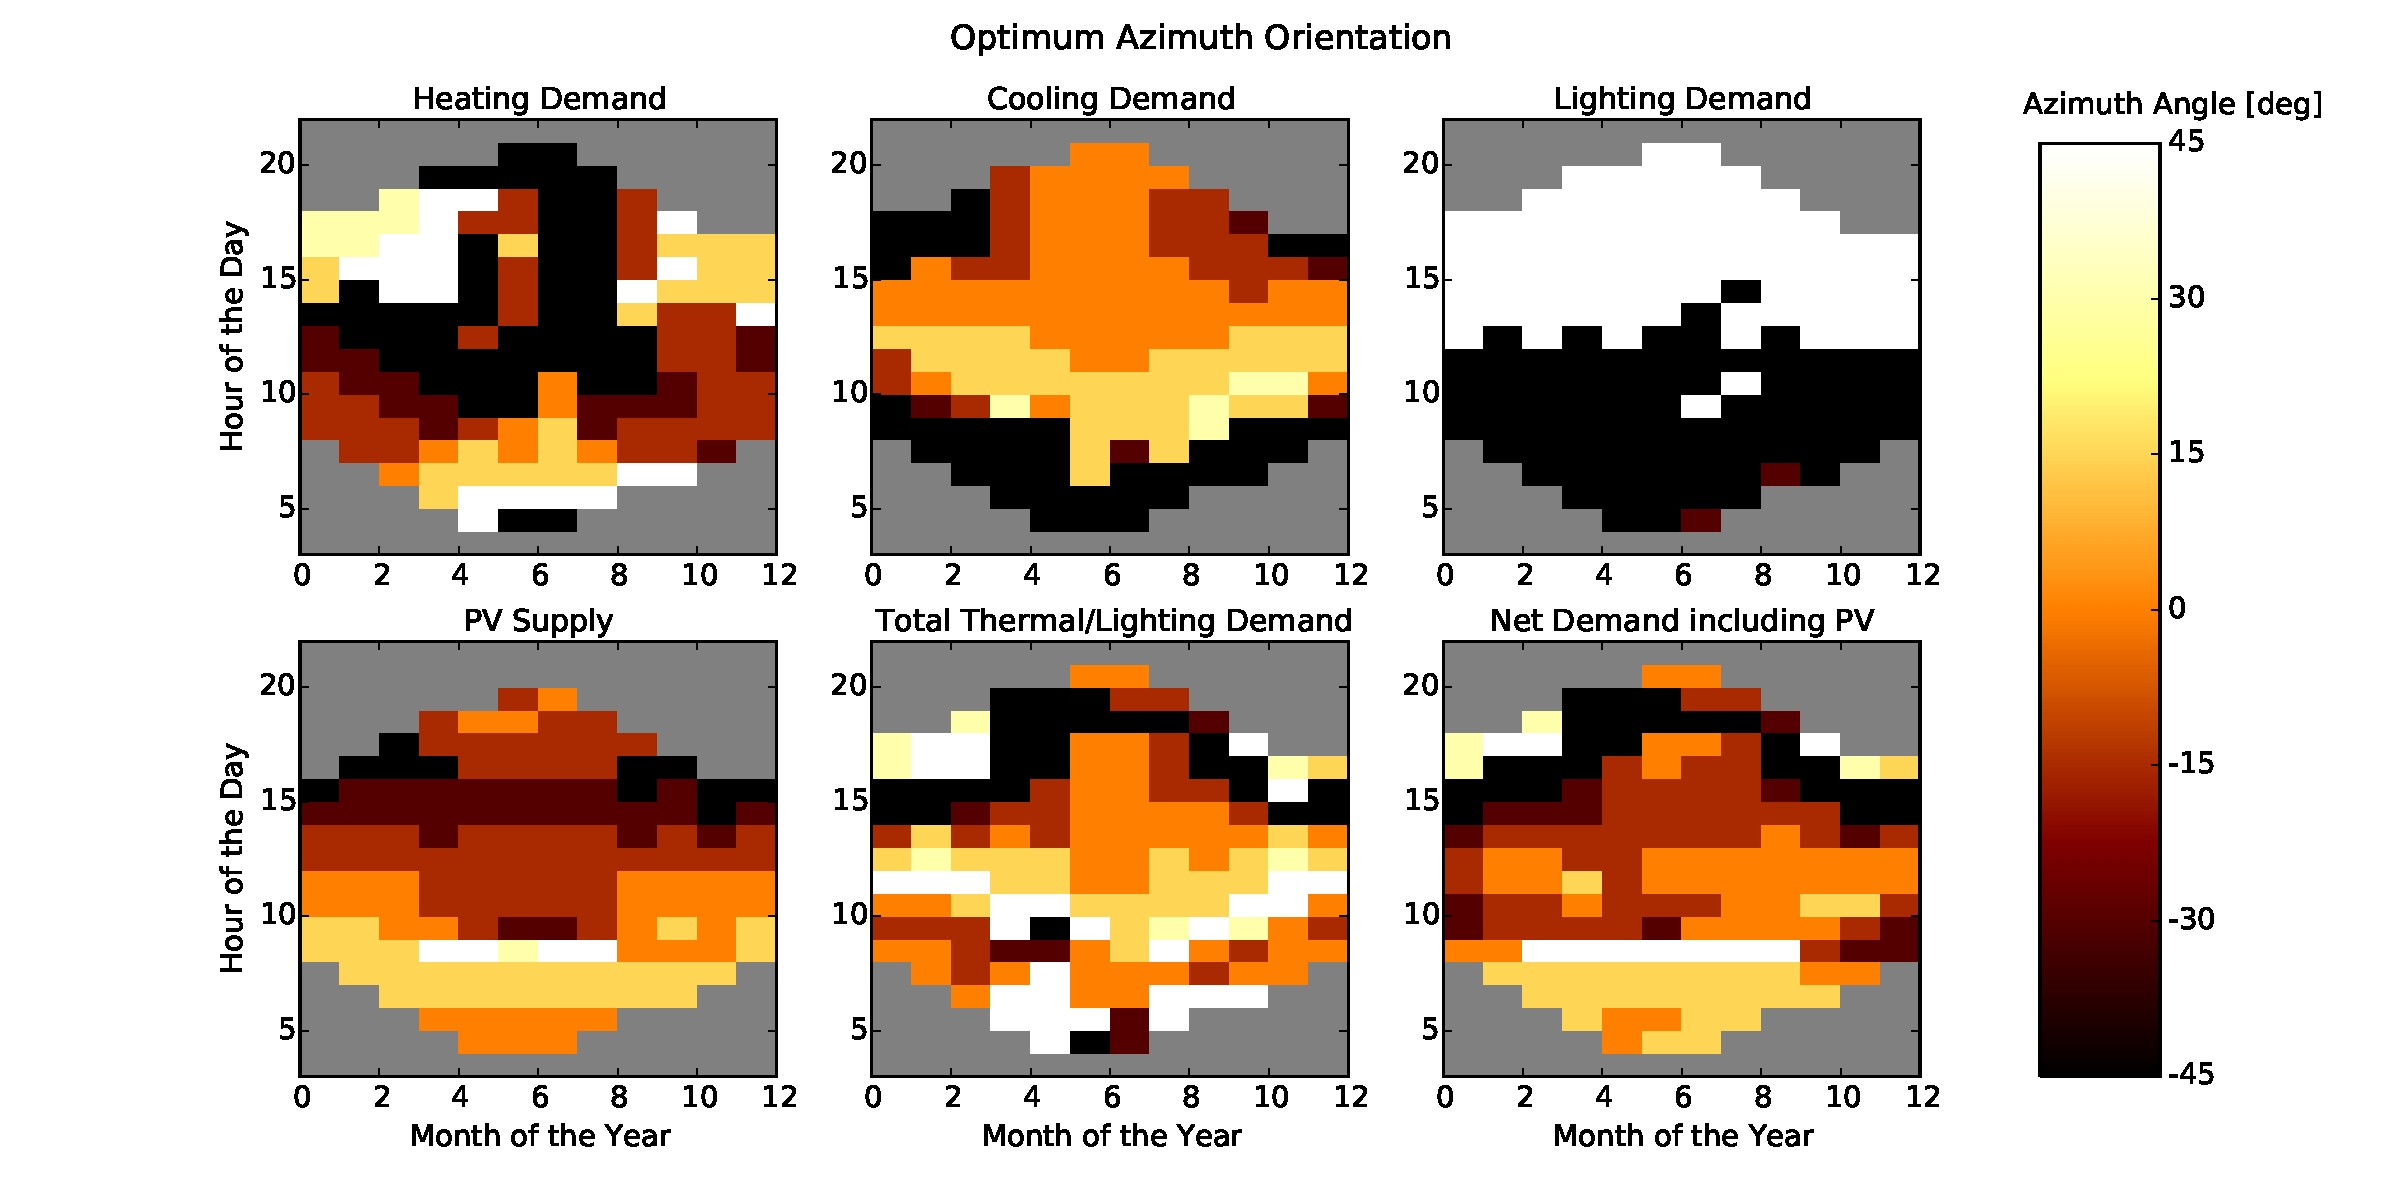
\includegraphics[width=\textwidth, trim= 1cm 0.5cm 1cm 1.4cm,clip]{monthly_azimuth}
	\caption{Carpet plots detailing the optimal azimuth angles to minimise the (a) heating demand, (b) cooling demand, (c) lighting demand, and (d) maximise PV electricity production. Figure (e) details the combinations for optimum building thermal management without PV production, (f) also includes the PV production. Negative angles correspond to the panels facing west, whereas positive angles represent east-facing panels. The corresponding altitude angles for each hour can be seen in the previous figure (\ref{fig:monthly_altitude}).}
	\label{fig:monthly_azimuth}
	\end{center}
\end{figure*}

In the altitude angle visualization it can be see that open configurations (light coloured) are chosen to minimise the building heating (a) and lighting (c) demand. Likewise, closed configurations (dark colours) are the preferred solutions to minimise the cooling demand (b). The PV optimisation tends to choose more open angles, corresponding to the minimization of longitudinal shading as will be described in section \ref{s:compareSunTracking}. In (e), the angles that optimise the overall building demand are shown. The optimisation chooses open positions at hours where heating and lighting is important, whereas closed positions are used for hours where cooling is dominant. The configurations for total energy minimisation - including the PV electricity production - are depicted in (f). It can be seen that there is a conflict in the summer evenings between minimising lighting and cooling demands. Likewise, there is a conflict between heating and PV production during the winter months. The overall energy optimization shows a strong tendency to follow the optimal PV production pattern. This, however changes if the building system becomes more inefficient. Less efficient heating for example, would result in configurations optimised for heating overpowering those of PV electricity generation.


Similar patterns can be seen for the azimuth variations. The azimuth angles correspond to the deviation from the building facade normal. Since the simulation was done for a south-facing facade, this means an angle with a positive sign represents the panels facing towards south-east (bright colours), whereas negative angles represent the panels facing towards south-west (dark colours). It can be seen that for heating and lighting, the facade takes positions that let the sun in, whereas for cooling the facade follows a sun-tracking pattern which prevents radiation to enter the room. The PV optimization also follows a sun-tracking pattern, though with a deviation towards facing east. This is caused by the PV-layout and the effects of longitudinal shading \cite{hofer2015PVSEC}. The optimization minimizes longitudinal shading in order to maximize PV electricity production. 

Figure \ref{fig:carpetplot_energy} shows the net energy use at these optimum angles. (a) shows that heating is mainly dominant in the winter and in the mornings, cooling (b) is primarily needed in the summer afternoons, lighting (c) at hours of low or no solar insolation, whereas PV electricity production (d) is dominant at hours with high solar insolation. (e) shows the total building energy demand and (f) visualizes the net energy demand including the PV electricity production. It can be seen that there is a net negative energy demand for most sunlit hours, meaning that the ASF is generating more energy than is used by the building for these hours. 

\begin{figure*}
	\begin{center}
	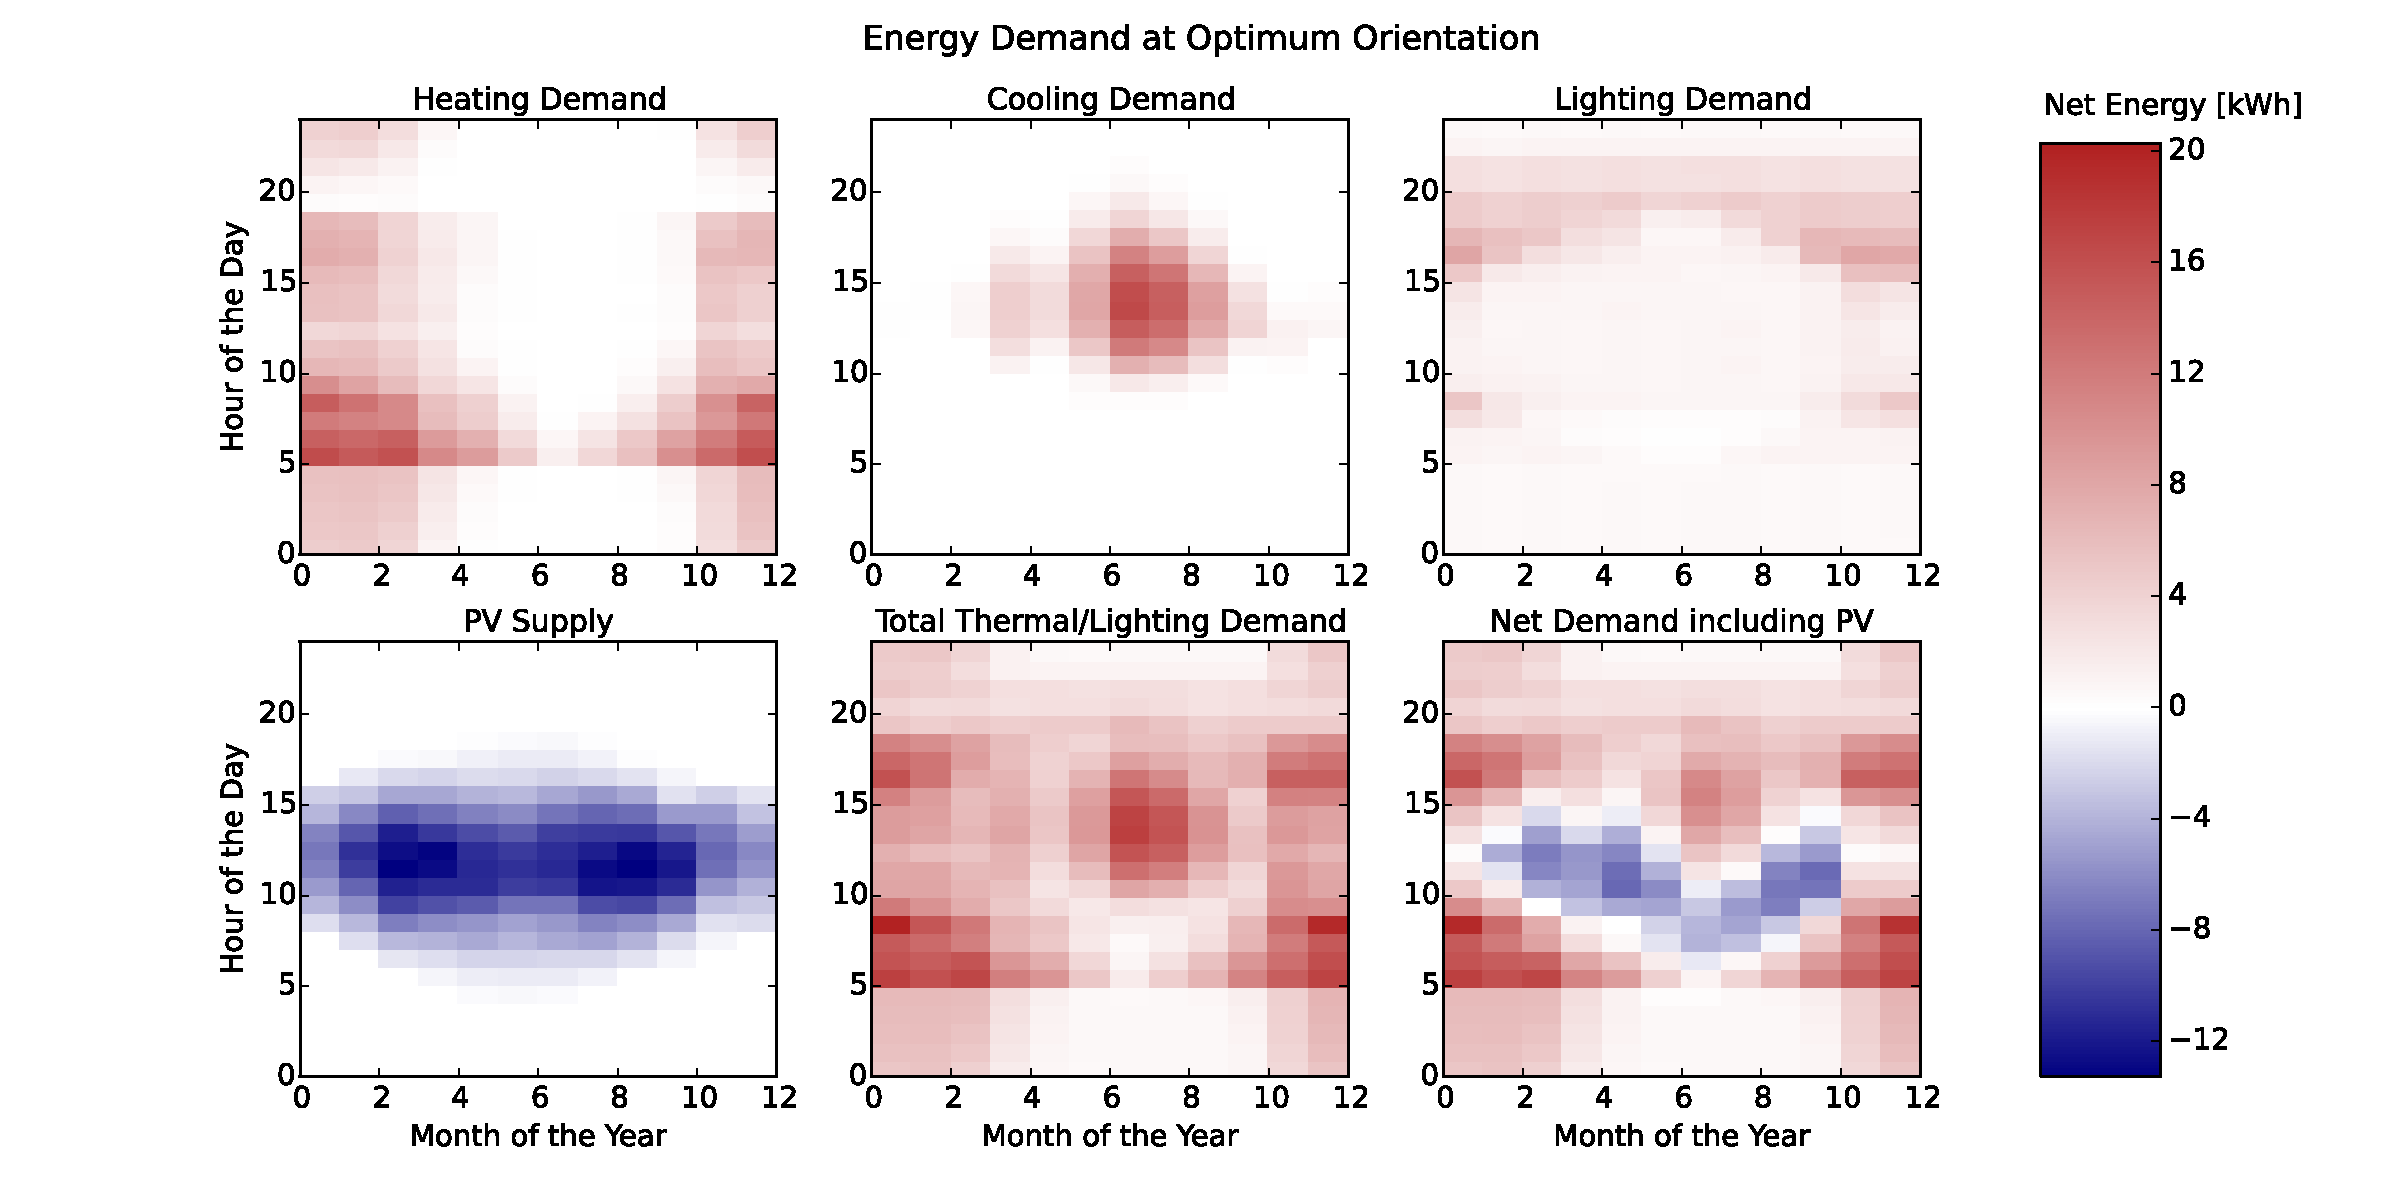
\includegraphics[width=\textwidth, trim= 1cm 0.5cm 1cm 1.4cm,clip]{monthly_energy}
	\caption{Carpet plots detailing the net energy consumption. Each square represents the total energy consumption for that specific hour of the entire month. Red colours detail the energy demand, while blue colours detail the energy supply.}
	\label{fig:carpetplot_energy}
	\end{center}
\end{figure*}


\section{Influence of Angle Actuation}
	In order to evaluate the influence of the actuation, three dimensional plots can be used to display all possible configurations and their corresponding energy benefit. In figure \ref{fig:3d}, the energy benefits of the altitude actuation are visualized for the months of March (a), June (b) and September (c). Each plot displays one cumulative day in hourly resolution. The x-axis  represents the altitude angles (19 different angles were evaluated with a step size of $5\degree$), the y-axis corresponds to the hour of the day, and the z-axis represents the energy benefit of the actuation, i.e. the difference in energy usage between the evaluated angle and the angle that yields the worst overall energy usage for each hour. It can be seen that the energy benefit is by far the largest around noon. Furthermore, positions that are rather closed tend to have the highest influence for the said mid-day hours. Open positions normally yield the worst benefits, except for some early morning or evening hours, where heating and lighting become important. This overall behaviour corresponds well to the results depicted in figure \ref{fig:monthly_altitude}, and shows why the angles that yield the optimum total energy, generally match the angles that optimize cooling and PV electricity production. A further interesting observation that can be made from this figure is the non continuous curves for midday hours. At an altitude angle of around $30^{\circ}$, the energy benefit reduces over proportionally. This is caused by the PV electricity production, larger angles will increase longitudinal shading and therefore over proportionally reduce the energy yield. 

	\begin{figure*}
		\begin{center}
		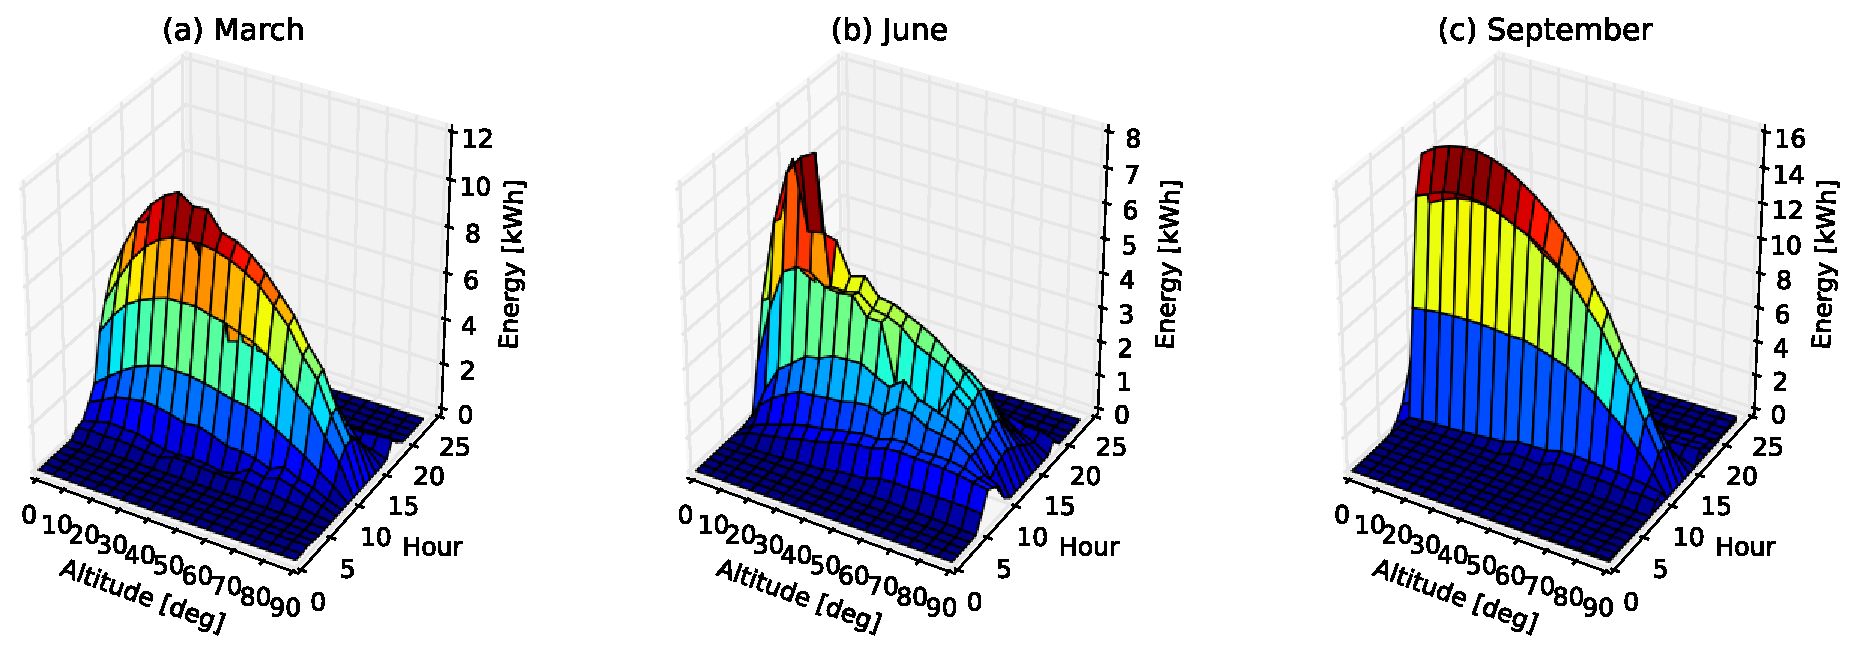
\includegraphics[width=1\textwidth, trim= 0cm 0cm 0cm 0cm,clip]{3d2}
		\caption{Energy benefits of the altitude actuation for the months of March (a), June (b) and September (c). Each plot displays one cumulative day in hourly resolution. The x-axis  represents the altitude angles, the y-axis corresponds to the hour of the day, and the z-axis represents the energy benefit of the actuation, i.e. the difference in energy usage between the evaluated angle and the angle that yields the worst overall energy usage for each hour.}
		\label{fig:3d}
		\end{center}
	\end{figure*}



%\section{Radiation and PV Analysis}

	
	%To evaluate the performance of the radiation simulation, a grid-convergence study was performed and the optimum grid size for further simulations was found. The radiation results could then be used to calculate the PV electricity production, enabling the finding of optimum angles to maximize PV electricity production. The corresponding energy output was finally compared to a control strategy using solar tracking.

	%\subsection{Grid Convergence}

		%With a larger grid-size, results are less accurate. In order to study this effect, a grid convergence study was conducted. Figure \ref{f:gridConvergence} shows the grid size dependency of the total radiation on the asf. The colors in the first two plots on the upper left represent the hours of the day. One can see in the second plot - where the radiation is normalized by a division with the radiation for a grid-size of 12.5\,mm - that the results are significantly more accurate for morning and evening hours. This is caused by increased self-shading at midday hours. The colours in the third plot on the left show the dependency on different combinations. No clear pattern could be found here. Finally the average deviation is depicted in the fourth plot on the left and a box-plot with all deviations is shown on the right. It can be seen that a smaller grid-size leads to larger deviations. While for a grid-size of 400\,mm the average deviation is over 10\%, the deviation goes down to below 1\% for a grid size of 25\,mm. 25\,mm was therefore taken as the grid-size of all simulations, as it gives accurate results, while still being computationally feasible. 

		%\begin{figure*}
		%	\begin{center}
		%	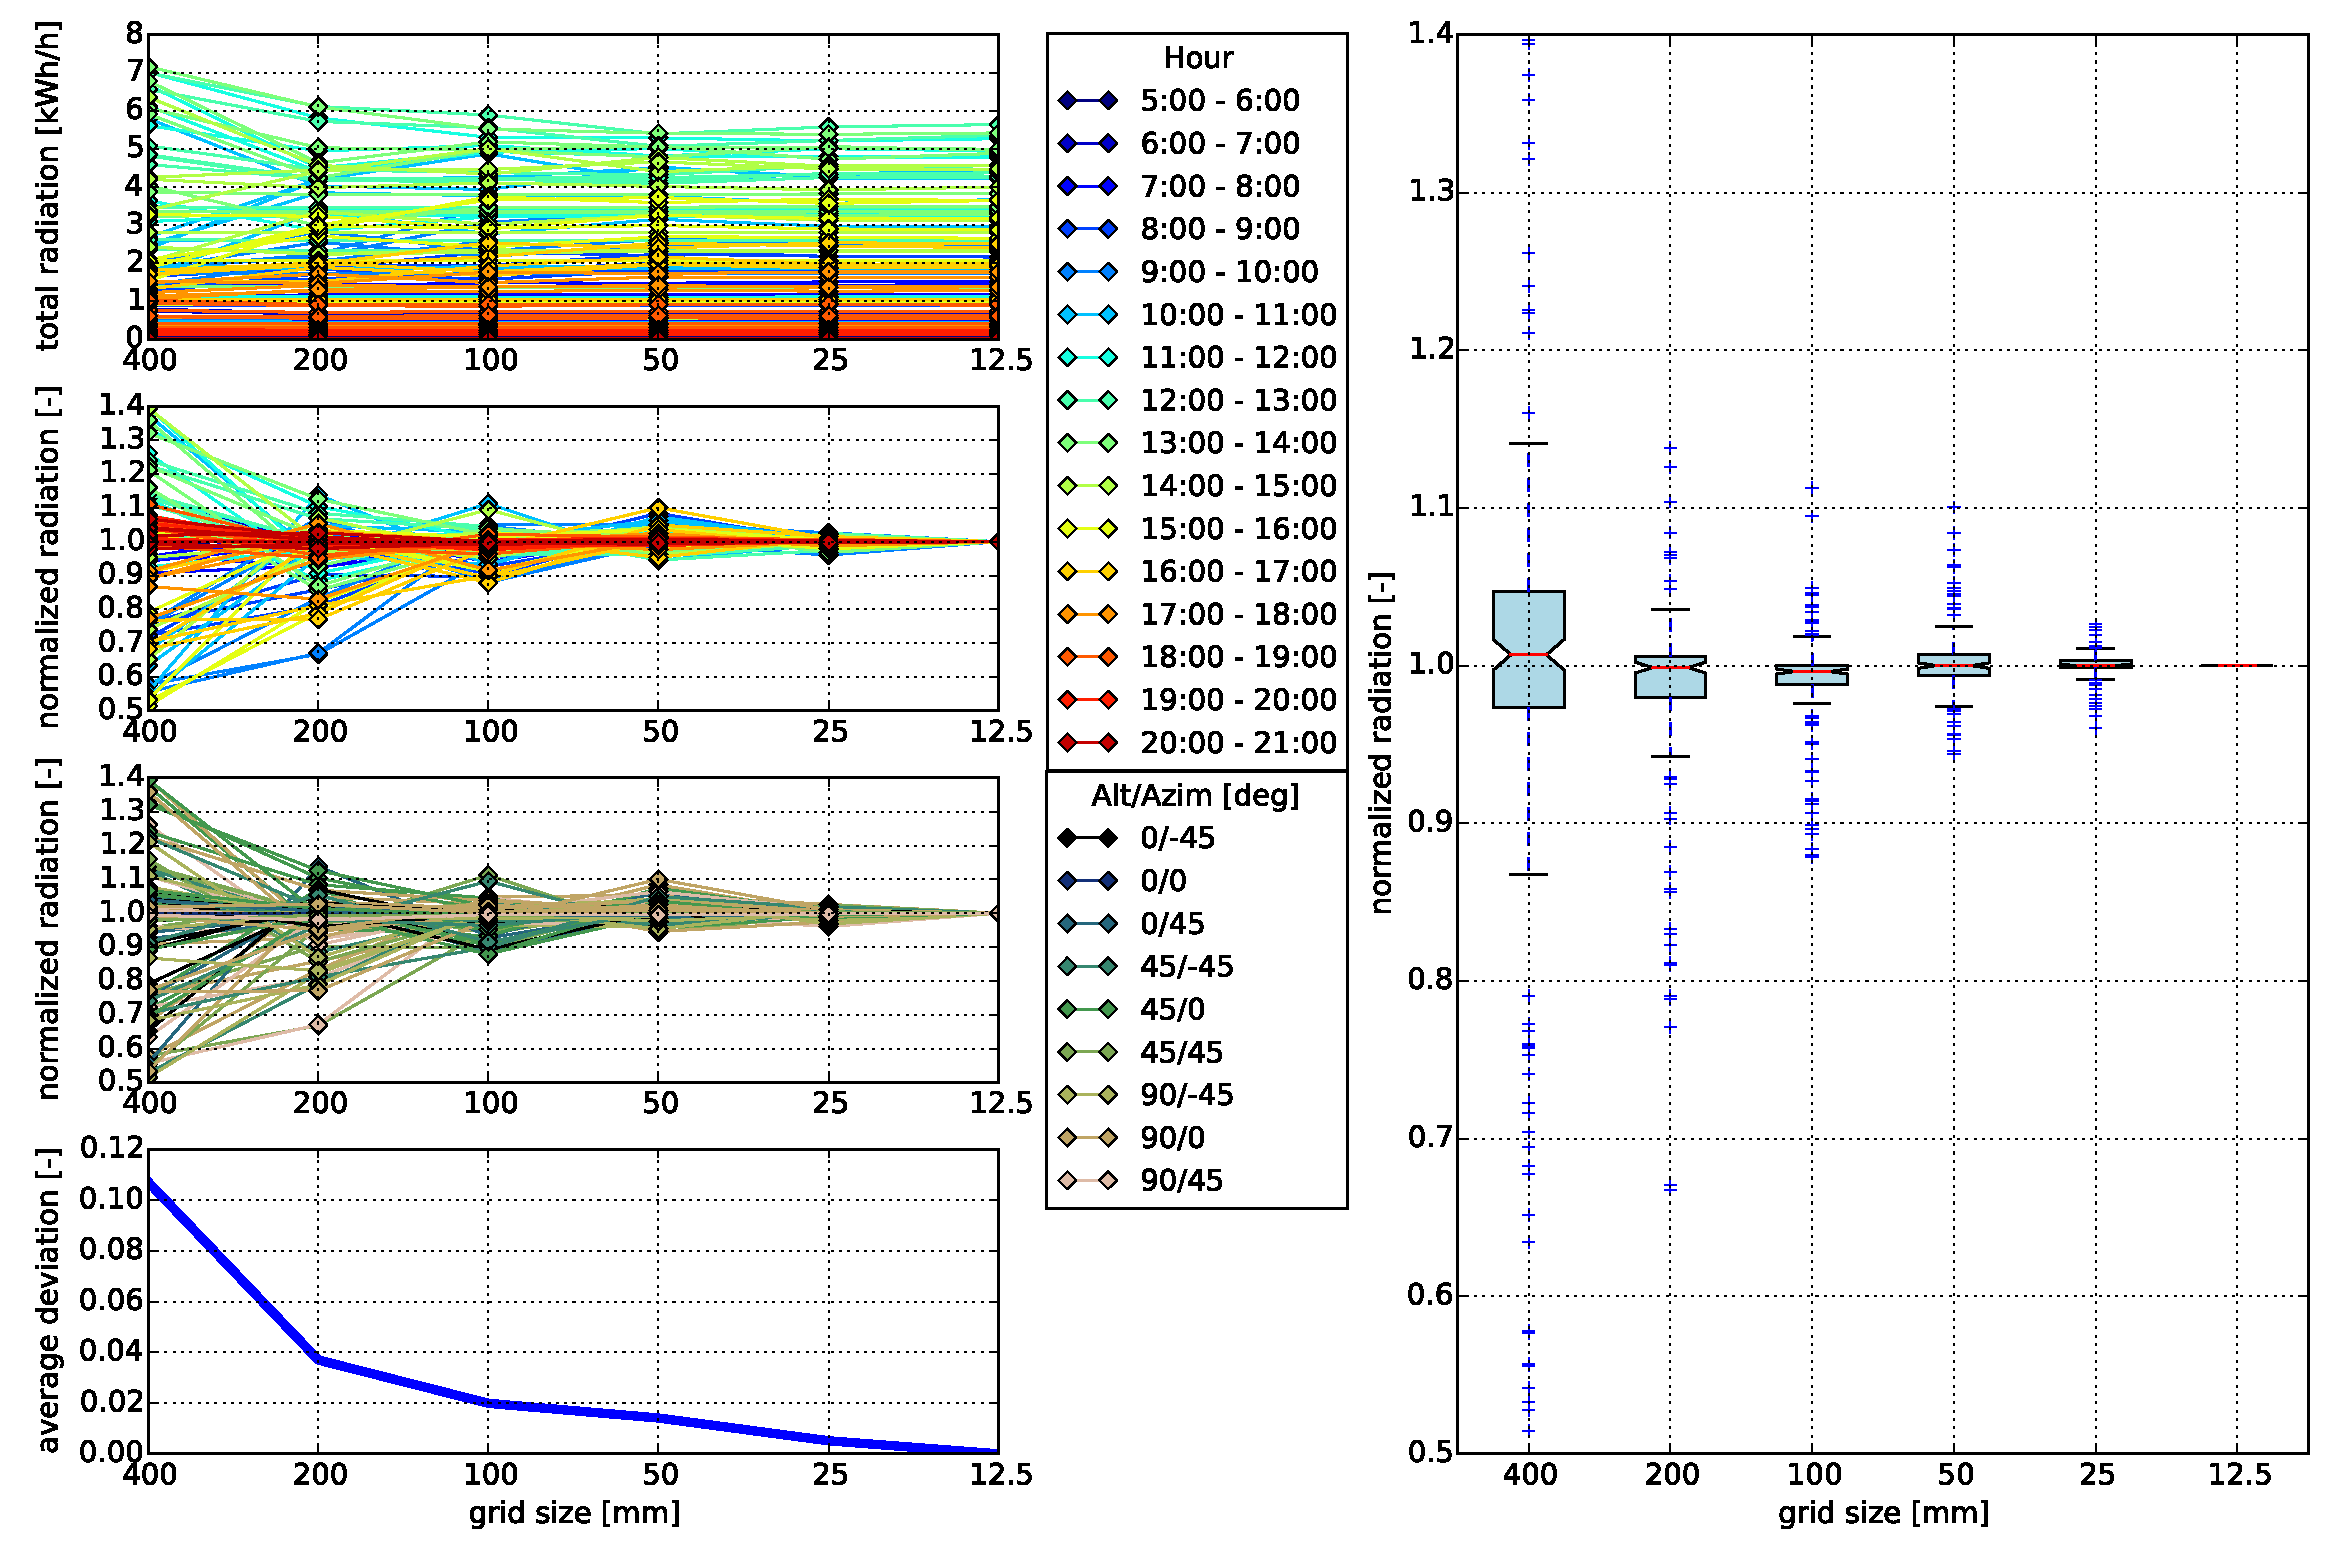
\includegraphics[width=\textwidth, trim= 0cm 0cm 0cm 0cm,clip]{gridConvergence.pdf}
		%	\caption{Grid convergence evaluation}
		%	\label{f:gridConvergence}
		%	\end{center}
		%\end{figure*}

	%\subsection{Comparison of Sun Tracking to Optimized Solution}
	%\label{ss:compareSunTracking}
\section{Comparison of Sun Tracking to Optimized Solution}
\label{s:compareSunTracking}

	In order to evaluate the optimum configuration for PV production, simulations using sun-tracking were compared to simulations evaluating 49 different combinations (i.e. 7 different azimuth and altitude angles). Figure \ref{f:compareSuntracking} shows the radiation on the panels in the first plot (a), also comparing it to the maximum radiation. The second plot (b) shows the PV electricity production for the two different control strategies, whereas the third plot (c) compares the corresponding efficiencies. It can be seen that while the radiation on the panels is pretty similar for both sun tracking and the optimized solution, there are very large losses in summer due to shading. Because of the shading, the total radiation on the panels is lower in summer than in spring and autumn. This can be explained by the higher altitude of the sun during summer months, the higher sun position results in increasing self-shading. Another observation is that the PV electricity production - as well as the corresponding efficiency - of the optimized solution is significantly higher than the sun-tracking solution in the afternoon hours. This is caused by the layout of the PV panels, longitudinal shading causes high power losses \cite{hofer2015PVSEC}, thus the optimized solution decreases the longitudinal shading compared to sun-tracking. Therefore, an optimizing solution should be preferred over a sun-tracking approach for control strategy considerations. Finally, the temperature dependency of the PV electricity model can be observed from the graph that is detailing the efficiency, even though the radiation in the winter months is significantly lower than during the rest of the year, the corresponding efficiency is comparatively high because of the lower temperatures in the winter months. 

	\begin{figure*}
		\begin{center}
		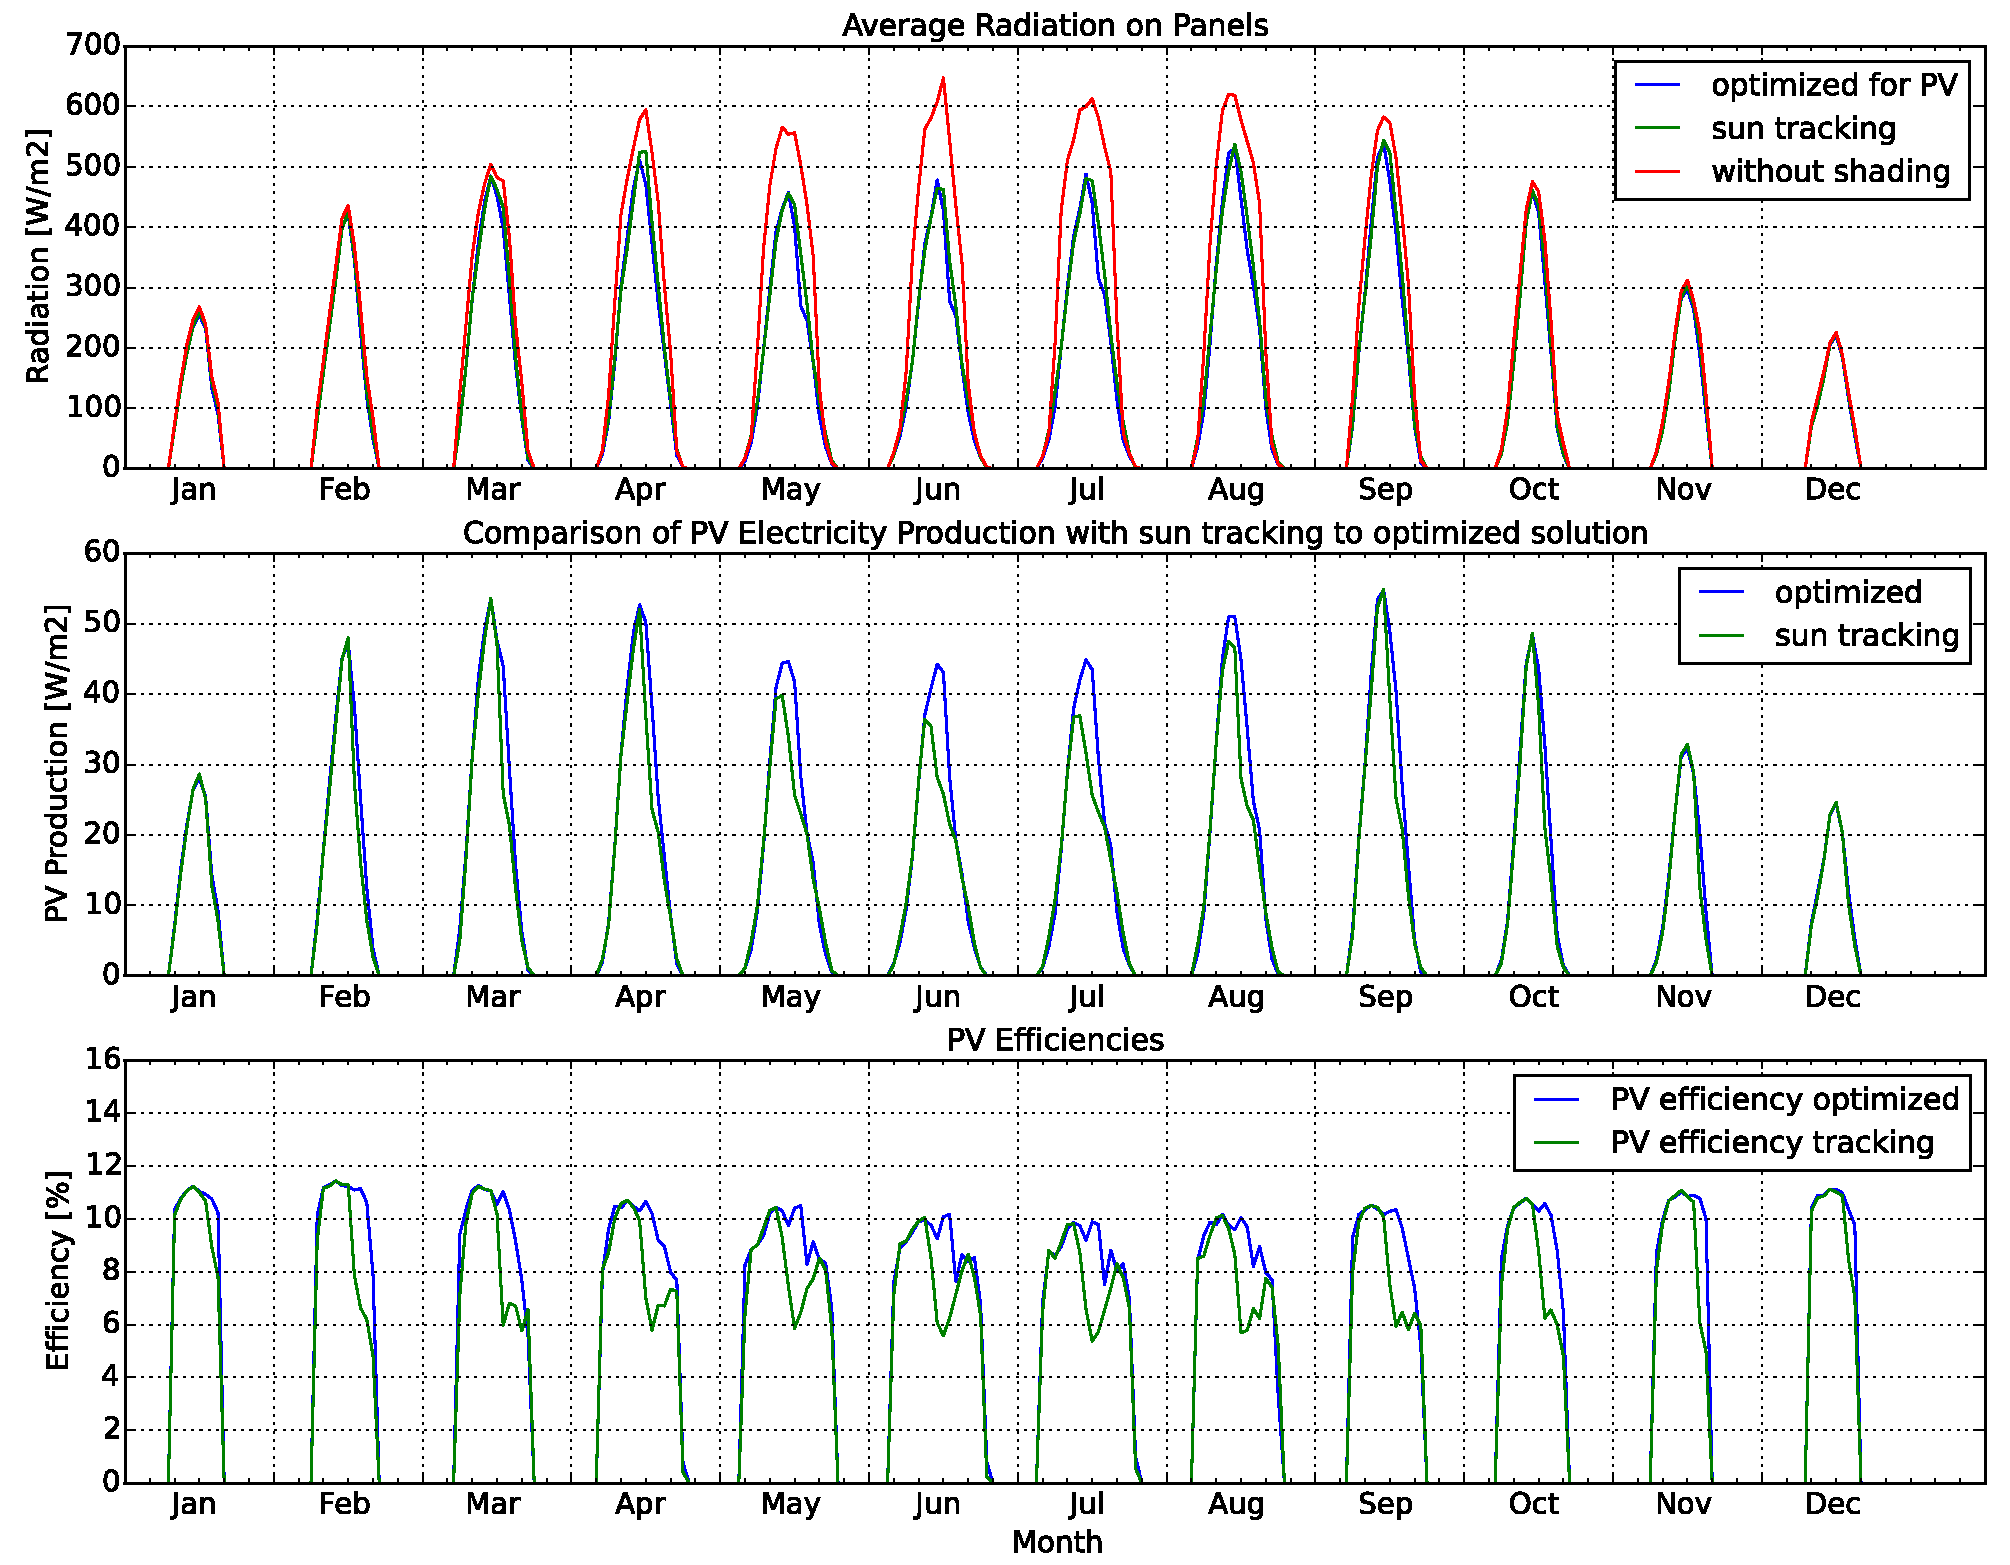
\includegraphics[width=\textwidth, trim= 0cm 0cm 0cm 0cm,clip]{PV}
		\caption{Comparison of optimized solution to sun-tracking. a) Average radiation on panels compared to radiation without shading. While the radiation for sun-tracking is very similar to the radiation with the optimized angles, there are large losses caused by shading. b) PV electricity production comparison. The optimized solution yields a significantly larger power output. c) PV efficiency comparison. The optimized solution is able to stay at higher efficiencies than the sun-tracking approach.}
		\label{f:compareSuntracking}
		\end{center}
	\end{figure*}



\section{Sensitivity on Control Strategy Approach}

	To evaluate further possibilities and limitations of the control strategy of the ASF, the tradeoffs between different strategies were visualised, as can be seen in figure \ref{fig:tradeoffs}. (a) shows the total energy demand used for heating, cooling, and lighting, the PV electricity production, as well as the total building demand and the net energy demand (building demand minus PV electricity production) for various control strategies. In (b) the corresponding differences in energy of the control strategy to the individually optimized solution is shown. As expected, the overall optimization is able to have the smallest deviations from the individually optimized results. When comparing the different control strategies, one can see that especially cooling and PV need to be optimized, while the heating and lighting demand have a lower sensitivity on the control strategy. Another observation that can be gained, is that the optimization for cooling is not very beneficial for the PV electricity production. This corresponds to the results in the previous section (\ref{s:compareSunTracking}), and is caused by the longitudinal shading, which naturally the cooling optimization does not take into account. However, the optimization for PV electricity production has a smaller negative influence on the cooling demand. This graph is part of the parametric simulation model, and can easily be adjusted to evaluate different building system parameters, as well as time periods. 

	\begin{figure*}
		\begin{center}
		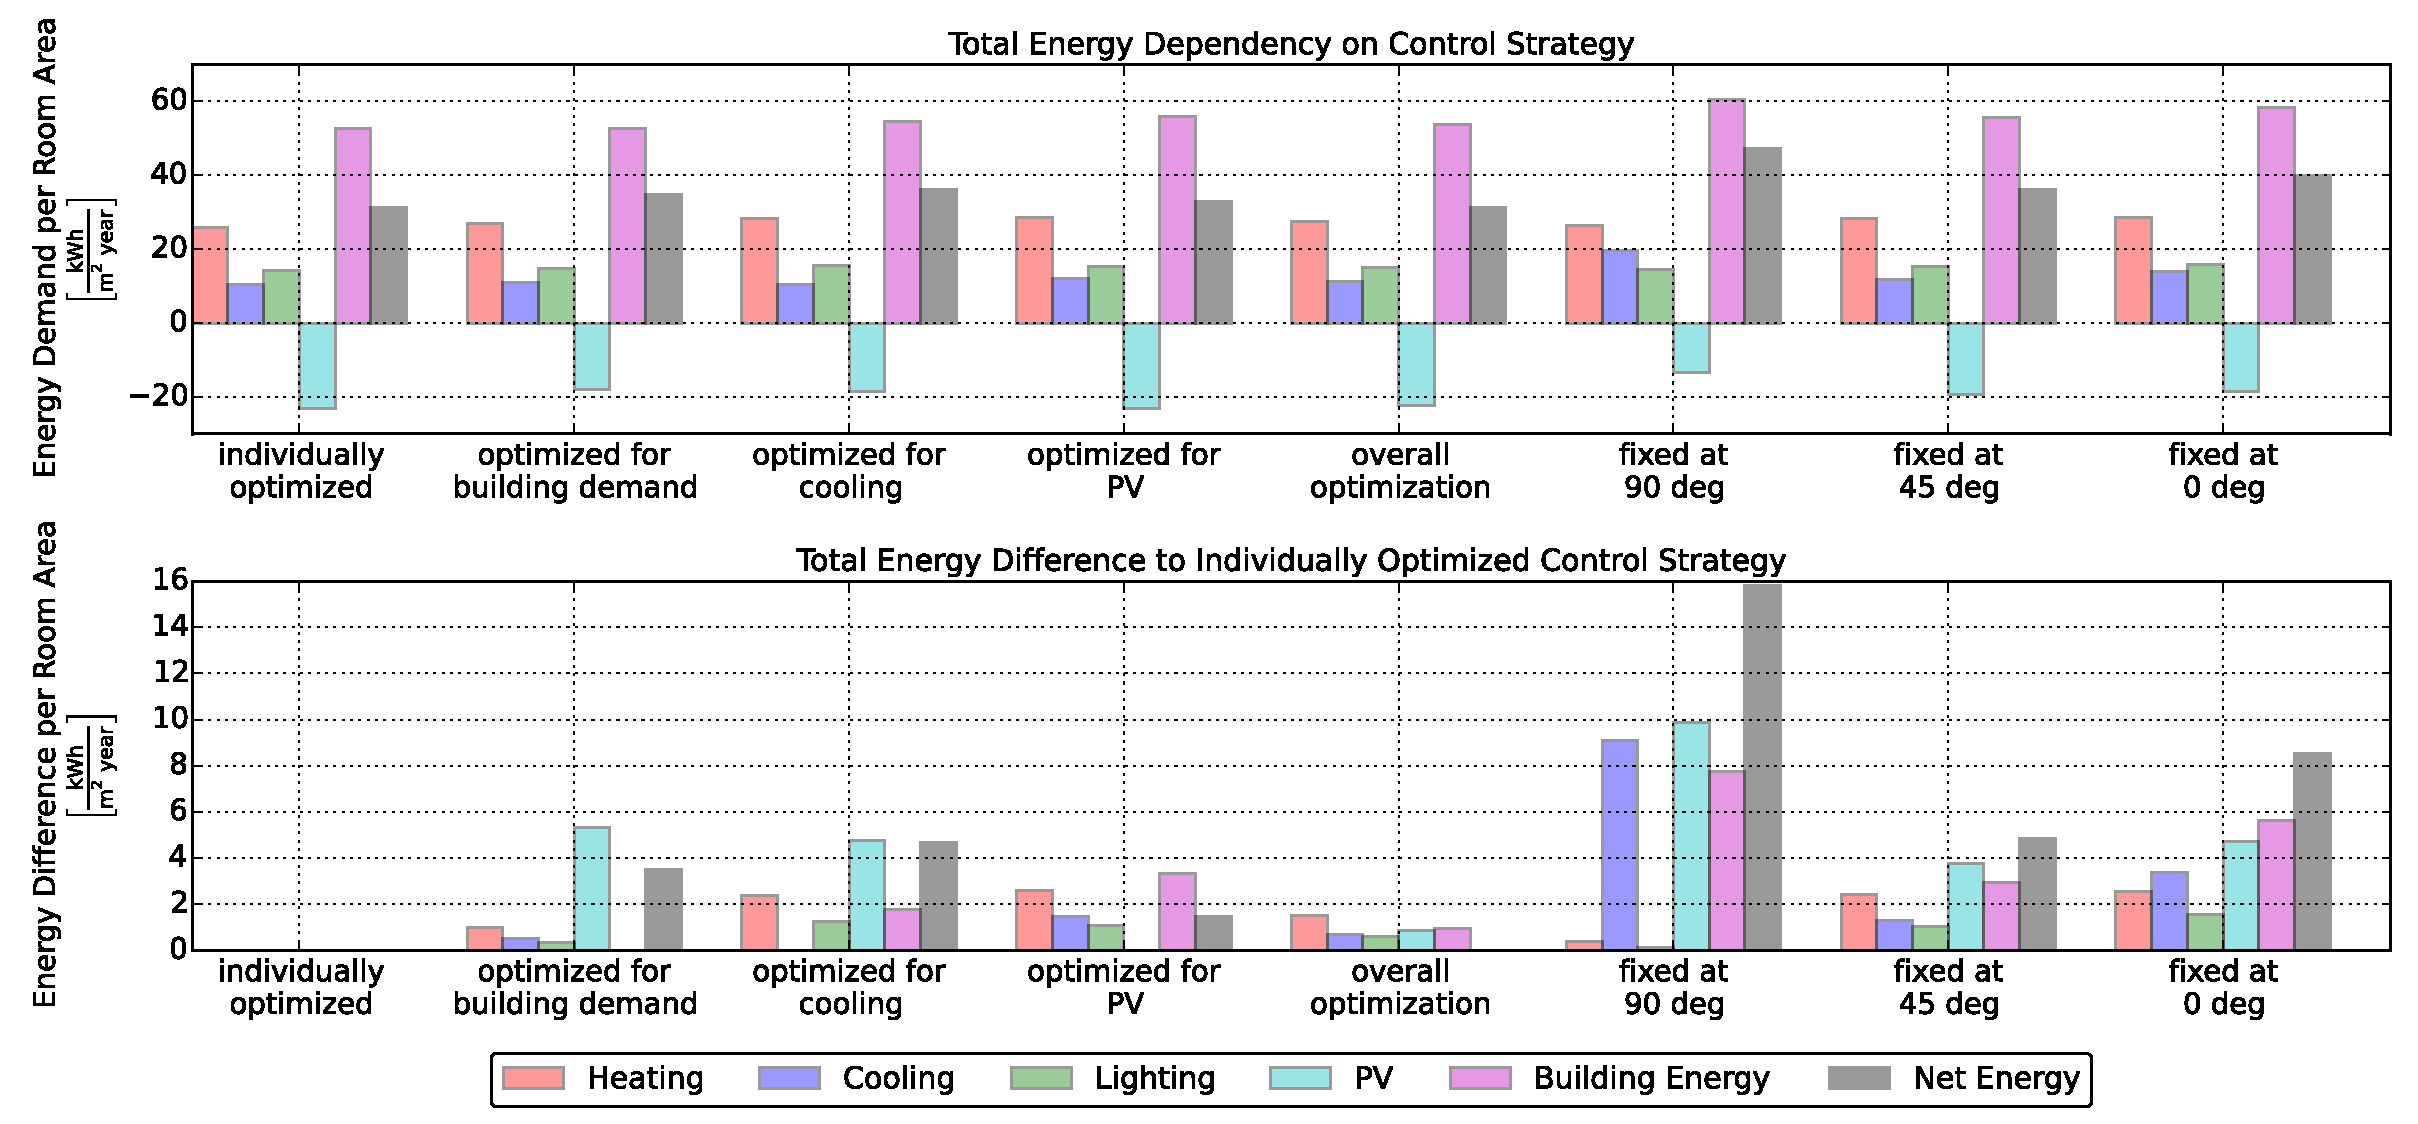
\includegraphics[width=1\textwidth, trim= 0cm 0cm 0cm 0cm,clip]{Tradeoffs}
		\caption{Comparison of different control strategies. (a) Total energy demand per room area. (b) Energy difference to individually optimized solution.}
		\label{fig:tradeoffs}
		\end{center}
	\end{figure*}


\section{Orientation Analysis}

	Evaluations of the facade for different building orientations were done with the base case of 5 azimuth and 5 altitude angles. Figure \ref{fig:buildingOrientation} shows the performance of the building and the facade for west, south-west, south, south-east and east orientations. (a) details the total energy demand for the optimzed solution, (b) compares the performance of the optimized solution to a fixed solar facade at a $45\degree$ altitude angle, and (c) compares the performance of the optimized simulation to a simulation without external shading. Non surprisingly, the south facing facade produces the most electricity. It also has the lowest building energy consumption, mainly because of low energy need for heating and cooling. It was found that the PV apertures should be oriented parallel to the upper left edge for facades that are west or south-west oriented, whereas they should be oriented parallel to the upper right edge for east or south-east oriented facades. This is caused by the shading patterns, longitudinal shading needs to be prevented as described in section \ref{s:compareSunTracking}. Furthermore, it can be observed that an east facing building uses less heating than a west facing building, which could be explained with the previous observation that heating is most important during morning hours. For similar reasoning the east facing building needs more cooling energy than the west facing building, because the room heats up in the morning and will not naturally cool down before outdoor temperatures drop in the evening. Interestingly, PV production is higher for the west facing facade than for the east facing facade. The cause for this is probably because of conflicts in optimizing cooling and PV electricity production at the same time, as cooling is more dominant for the east facing building. Overall, the south-east facing facade performs the best, when compared to the corresponding reference cases. It can clearly be seen, that this performance increase mainly comes from the high cooling demand, the benefits of the facade for the cooling electricity outweigh the lower benefit in PV electricity supply. 
	\begin{figure*}
		\begin{center}
		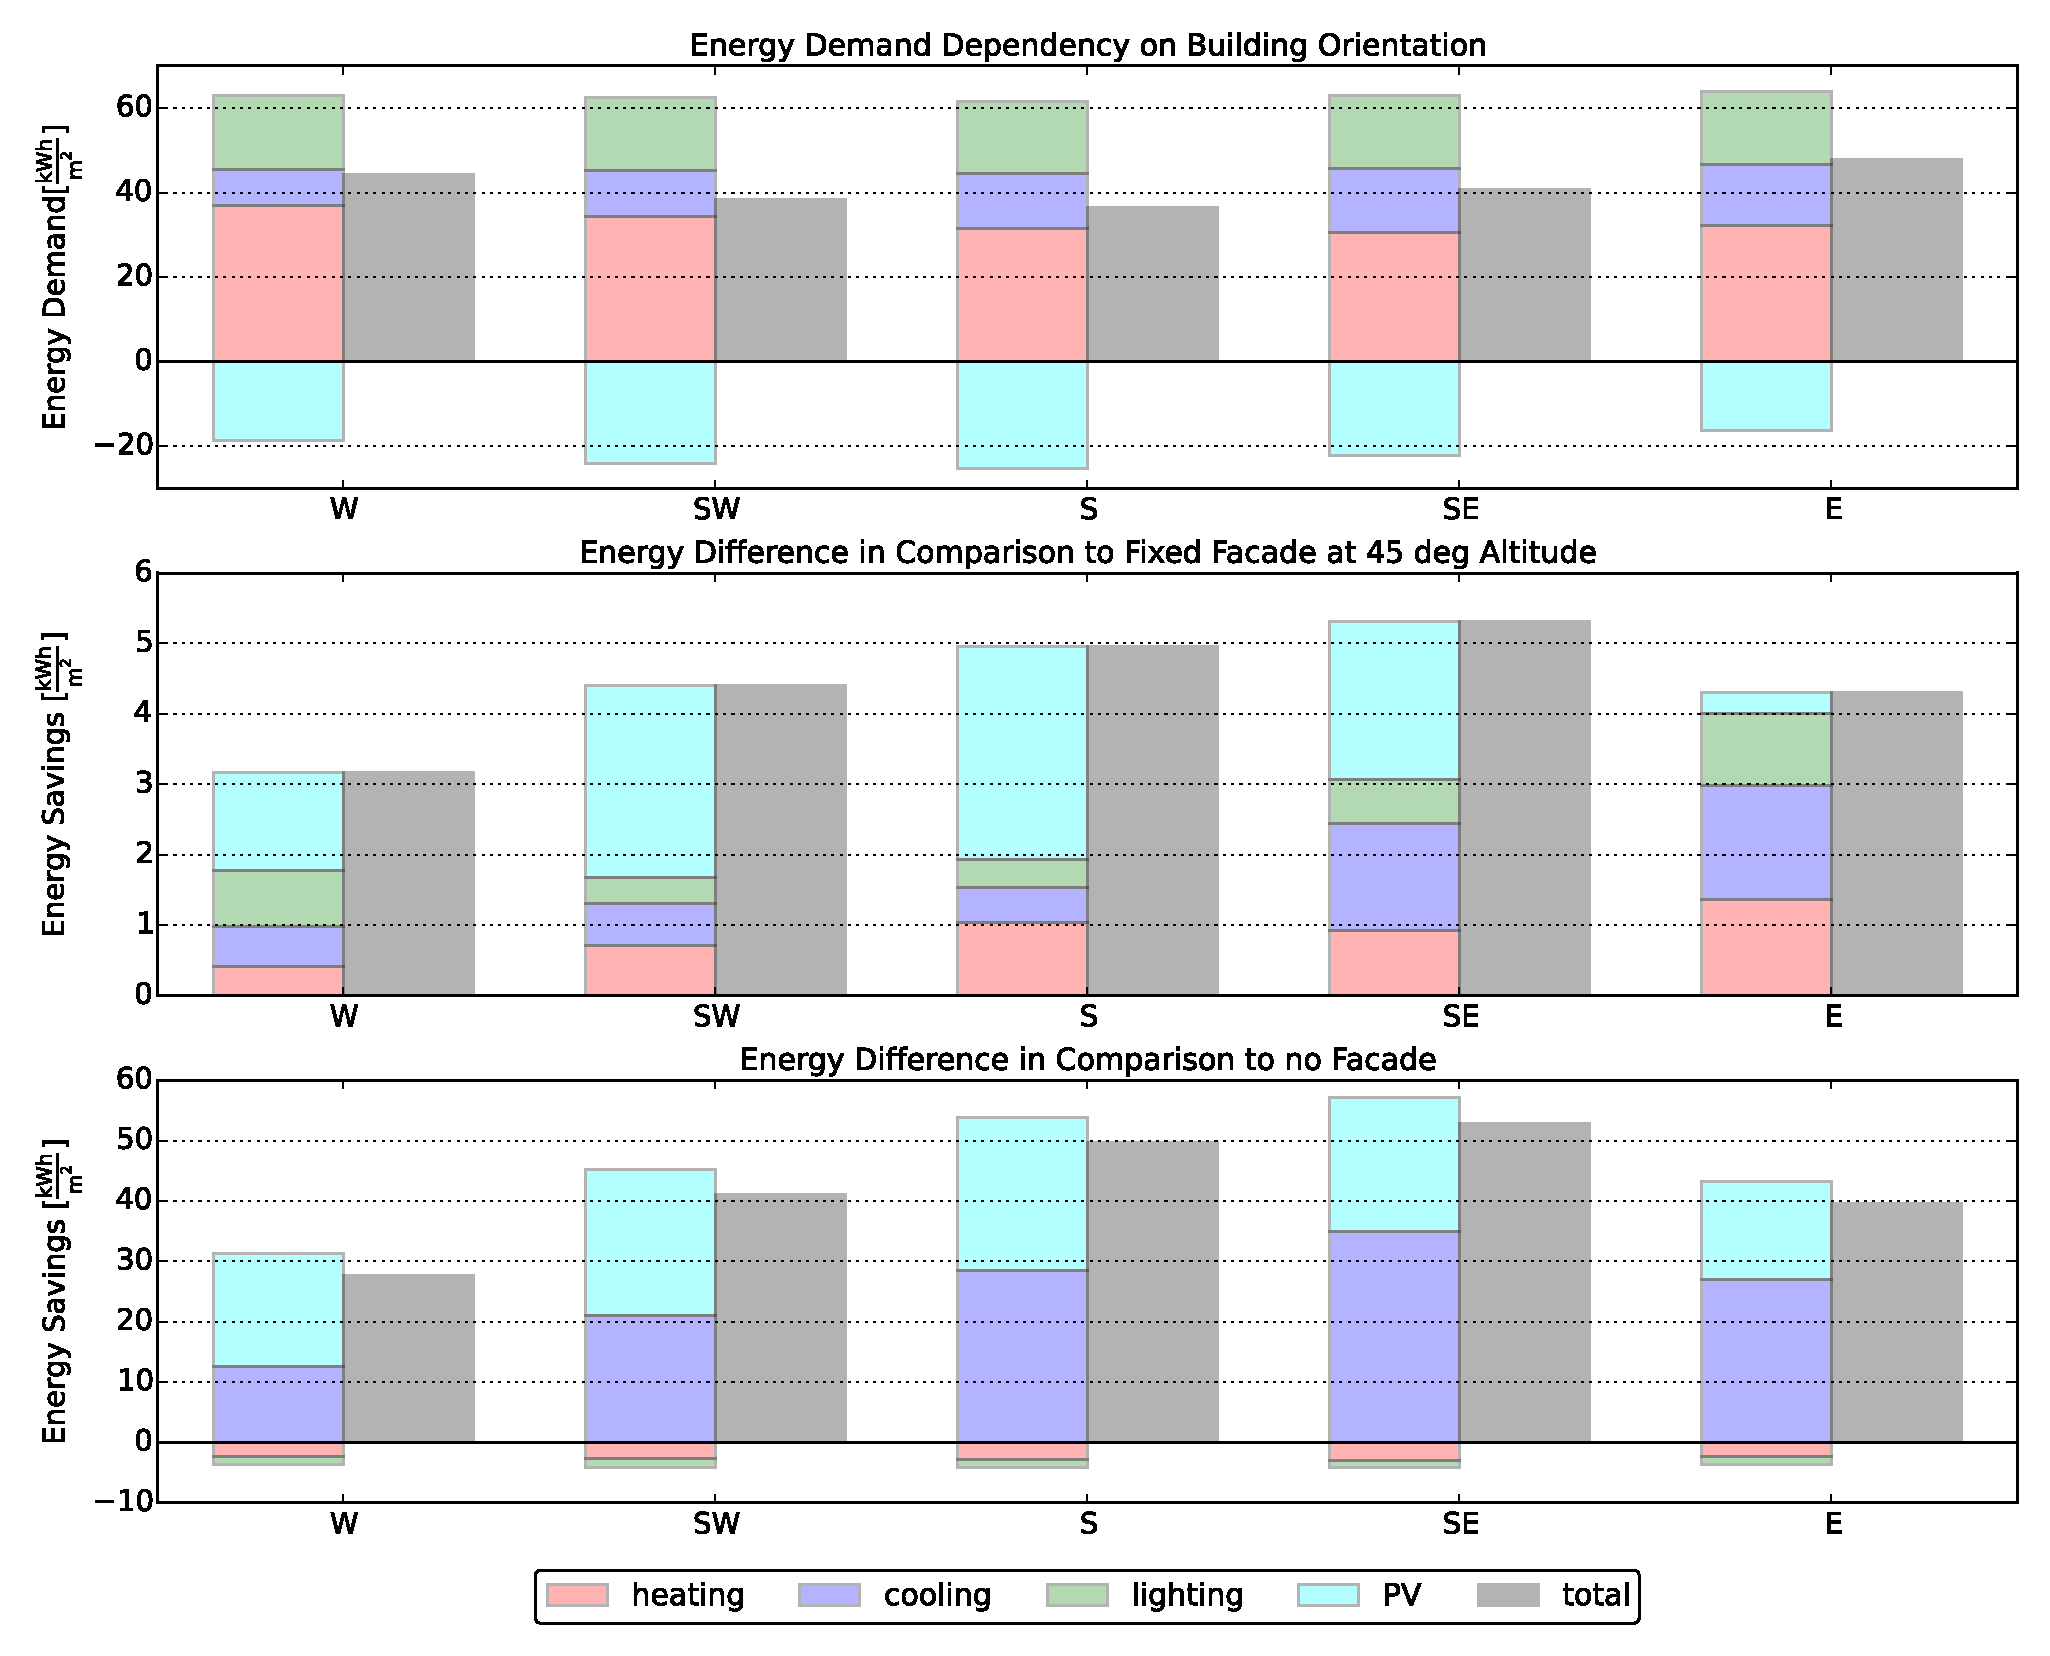
\includegraphics[width=\textwidth, trim= 0cm 0cm 0cm 0cm,clip]{orientation}
		\caption{Energy demand in dependence of building orientation. South facing facades perform best.}
		\label{fig:buildingOrientation}
		\end{center}
	\end{figure*}


\section{Location Analysis}

	Similarly to the orientation analysis, the location of the building was evaluated. In figure \ref{fig:buildingLocation}, the corresponding energy performance of an ASF is shown for the loactions Helsinki, Zurich, Madrid, and Cairo. 

	\begin{figure*}
		\begin{center}
		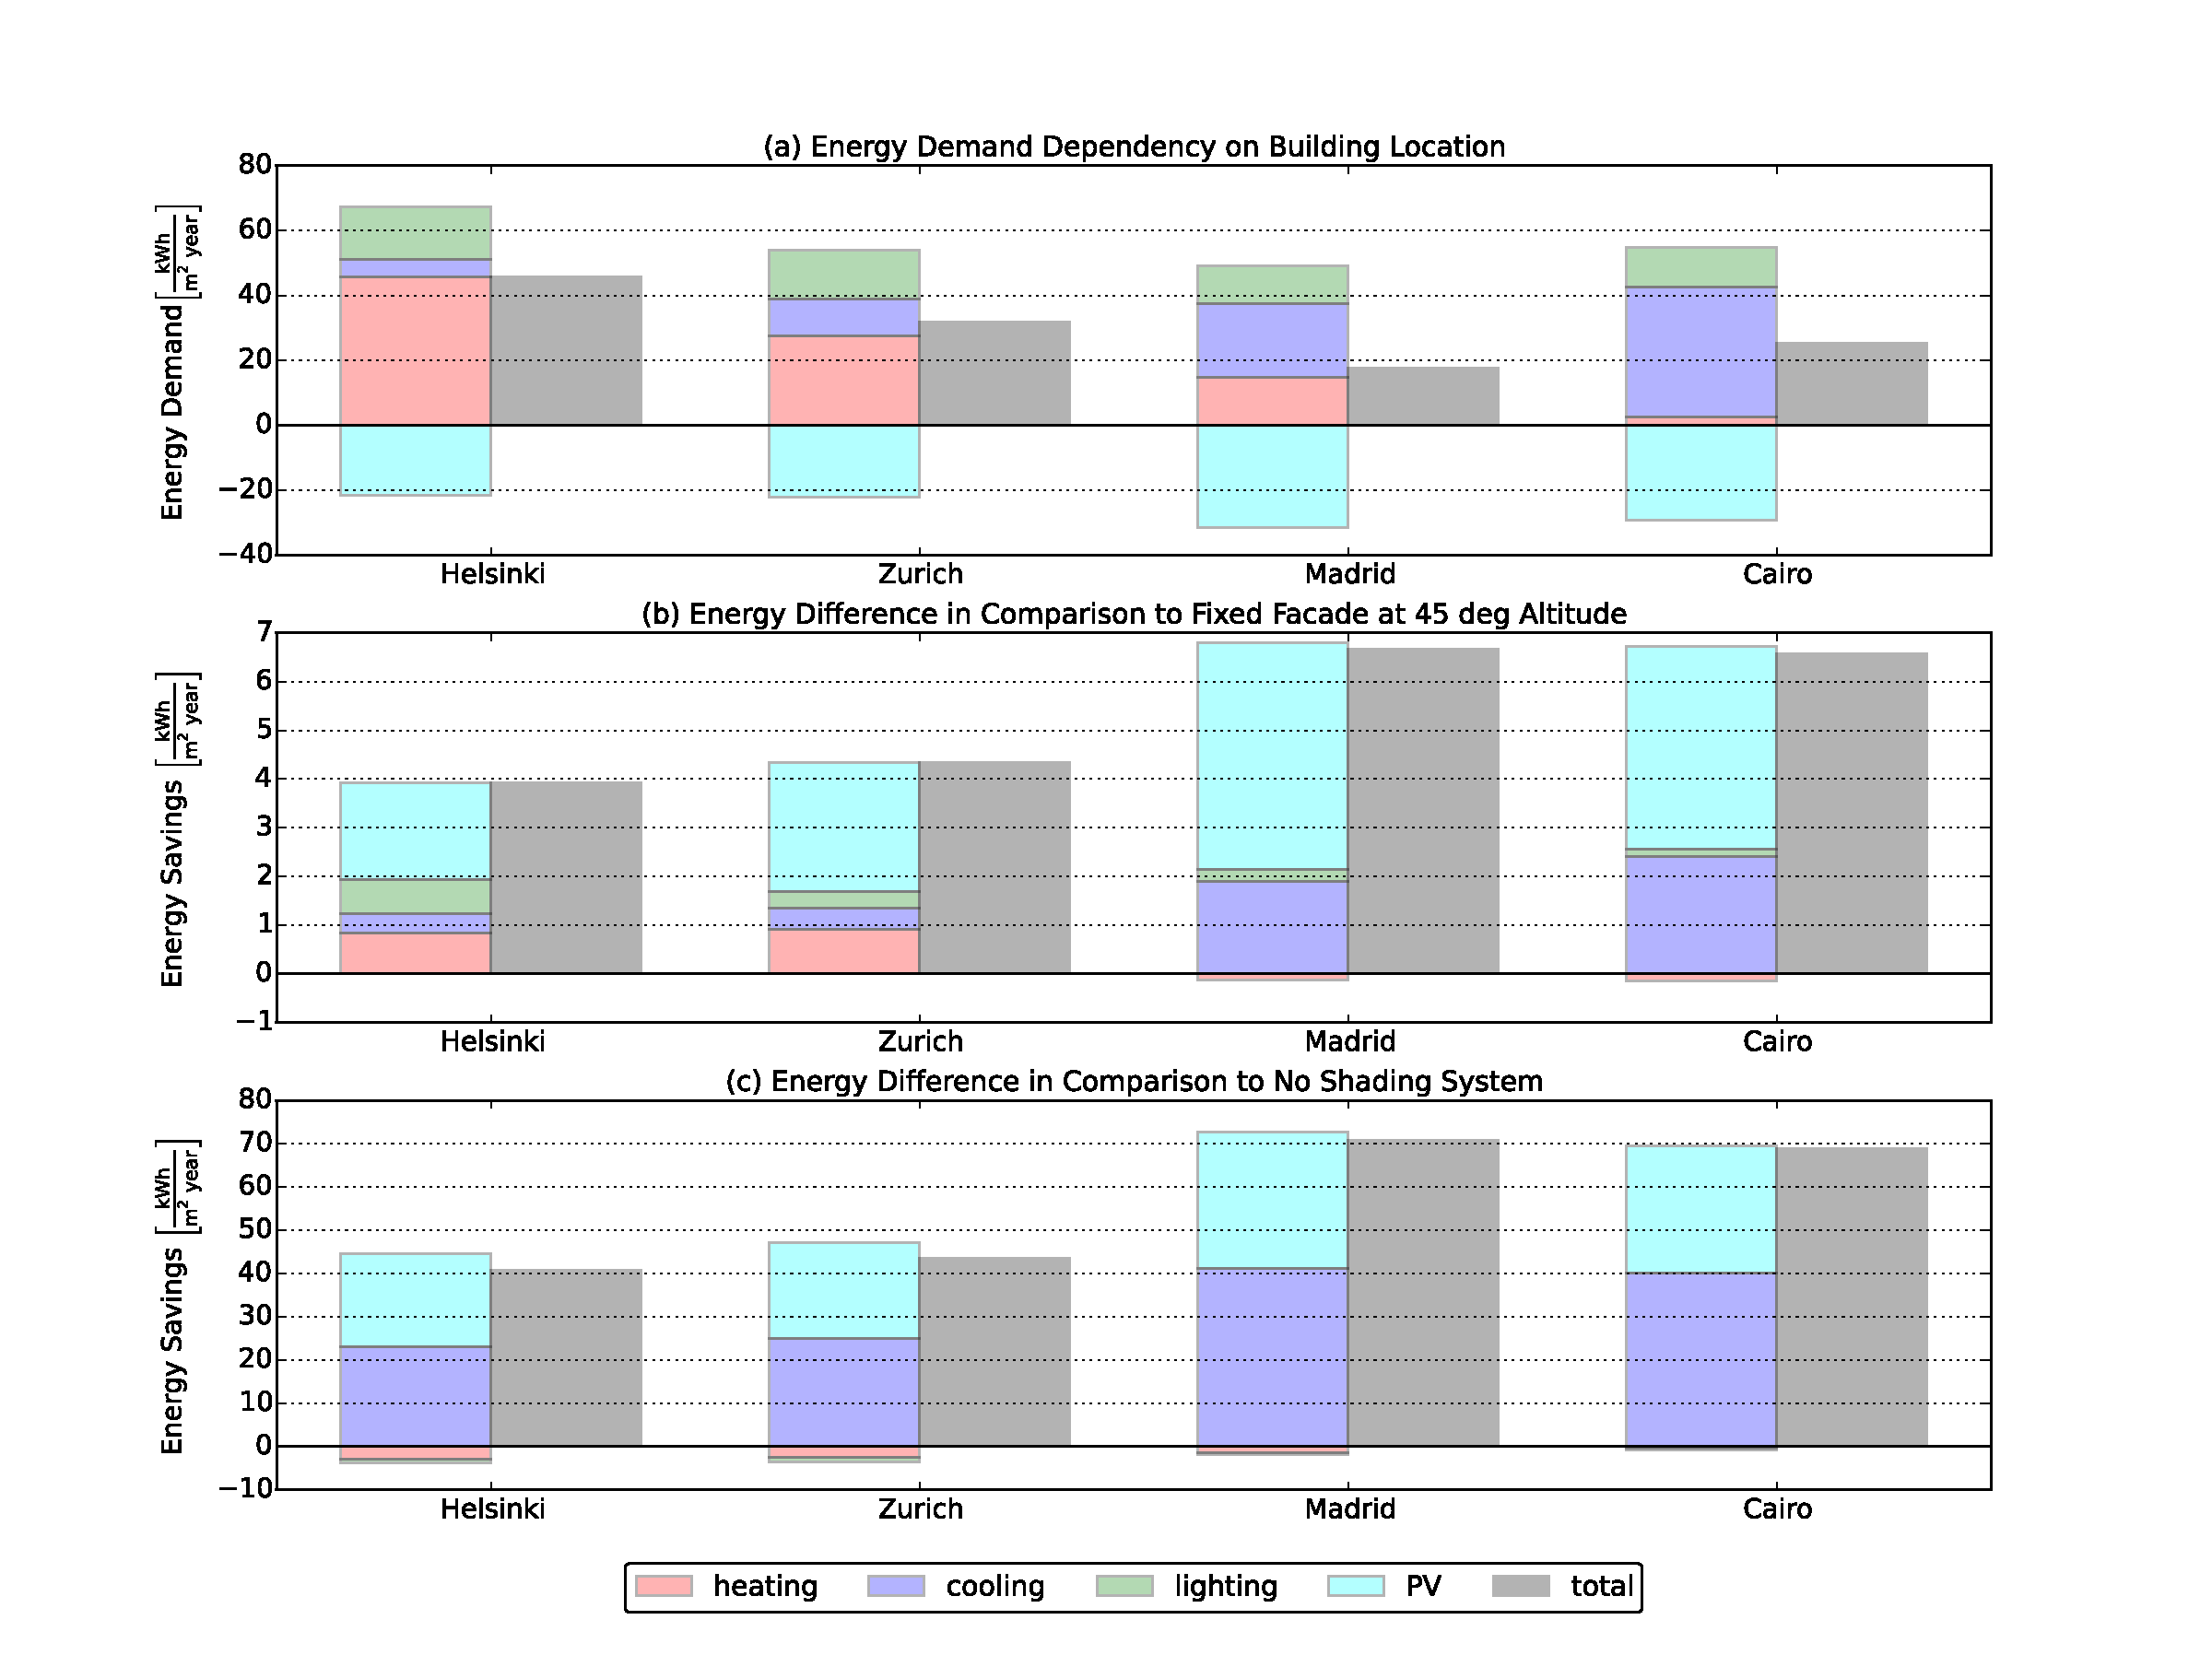
\includegraphics[width=\textwidth, trim= 0cm 0cm 0cm 0cm,clip]{Location}
		\caption{Energy demand in dependence of building location. Best performance for warm and sunny regions.}
		\label{fig:buildingLocation}
		\end{center}
	\end{figure*}
\section{Sensitivity on Building System Parameters}

	A sensitivity analysis was done for heating COP, cooling COP, lighting load, average PV efficiency, building orientation, infiltration rate and combination variations for the time period of one year. The results are shown in figure \ref{fig:sensitivity}. The top row shows the energy savings per square meter of room area compared to a fixed solare facade at an angle of 45\degree, whereas the bottom row shows the energy savings compared to a building without any PV modules or shading devices. 

	\begin{figure*}
		\begin{center}
		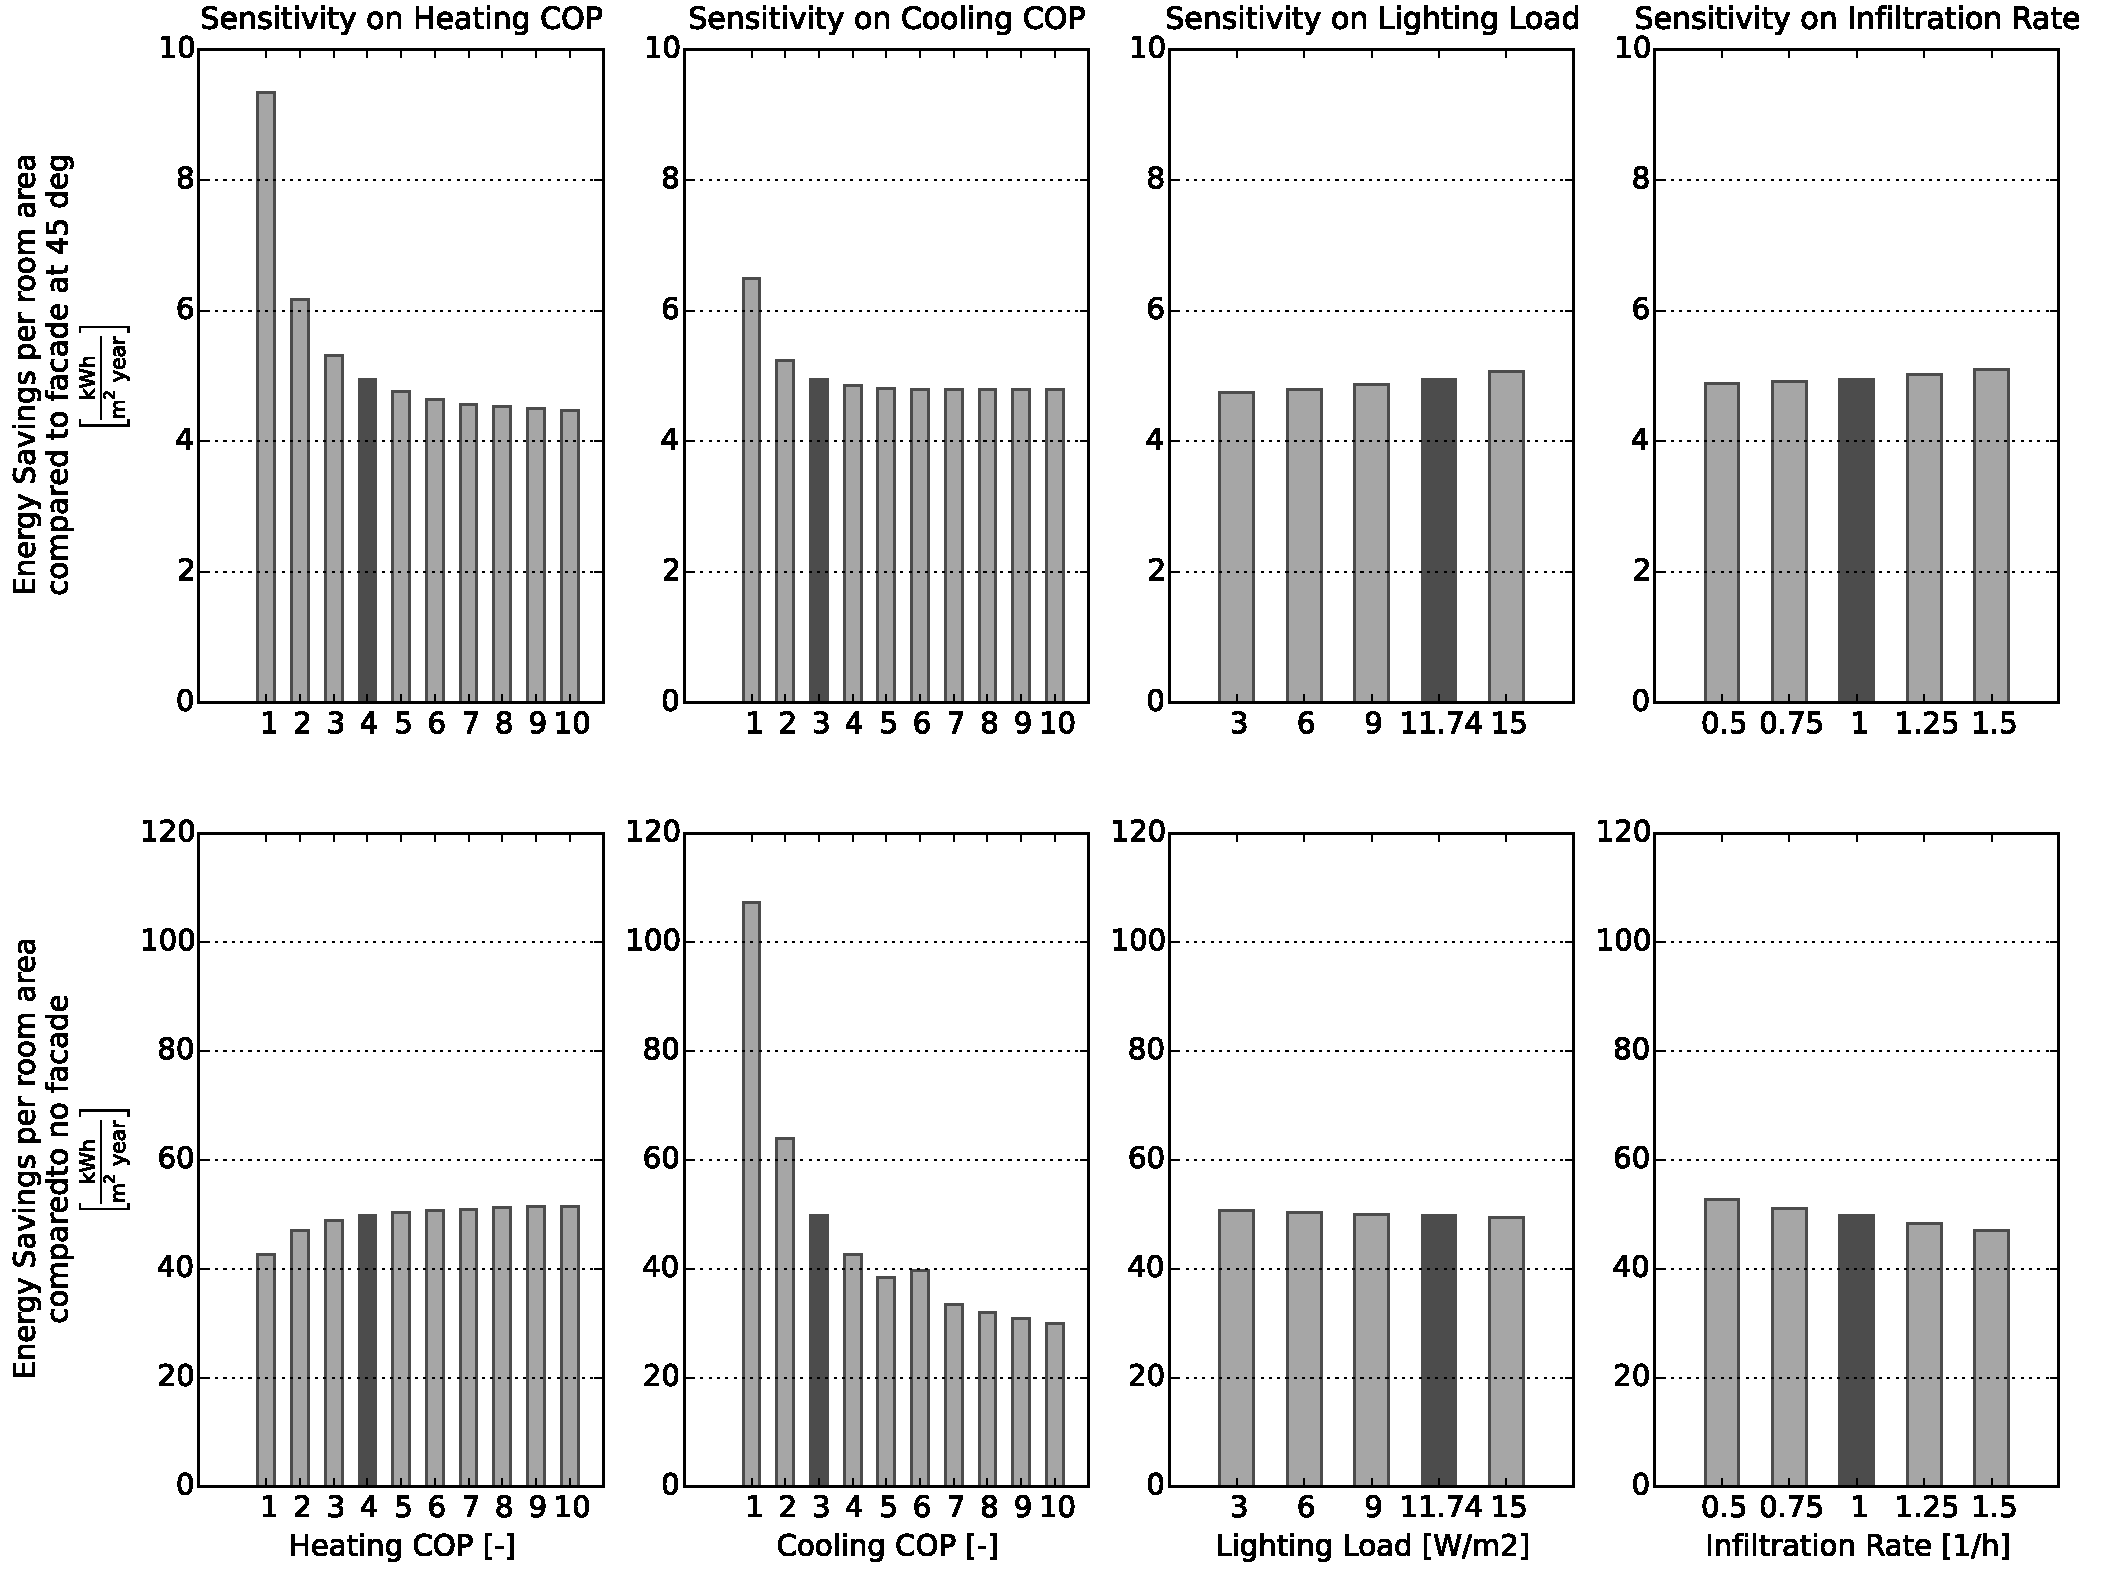
\includegraphics[width=\textwidth, trim= 0cm 0cm 0cm 0cm,clip]{buildingSensitivity}
		\caption{Sensitivity analysis of energy savings during one year. From left to right, sensitivities on heating COP, cooling COP, lighting load, average PV efficiency, building orientation, combination variations and infiltration rate. Top row shows the energy savings compared to a fixed solar facade at a 45\degree altitude angle, the bottom row shows the energy savings compared to a room without shading or PV modules.}
		\label{fig:sensitivity}
		\end{center}
	\end{figure*}

\section{Evaluation of Different Combination Settings}
	
	With the parametric model, it is possible to evaluate every thinkable set of angle combinations. However, computational limitations require a discrete set of angles. In order to assess the influence of the chosen angle combinations on the performance of the ASF, various different combinations have been evaluated. In figure \ref{fig:combinations}, the energy savings of various simulation combinations are shown, compared to a fixed solar facade at a $45\degree$ altitude angle (a), as well as to a building without external shading (b). Variations include evaluations of using only one axis actuation (i.e. either a fixed azimuth or a fixed altitude angle), as well as using multiple angles for both altitude and azimuth actuation. The angles were always distributed equally between $0\degree$ and $90\degree$ or between $-45\degree$ and $45\degree$ for the altitude and azimuth variations, respectively. When using multiple angles, the maximum and minimum actuation angle was always included. For example an analysis using three altitude and three azimuth angles was using $0\degree$, $45\degree$ and $90\degree$ for the altitude variations, while the azimuth variations would include the angles $-45\degree$, $0\degree$ and $45\degree$. It can be seen that the more angles are used, the higher the energy savings become. However, with an increasing number of combinations comes a corresponding increasing amount of computation time. Higher energy savings will definitely be possible with the use of an increasing number of combinations, though the benefit of increasing the number of combinations will gradually go down to zero. 
	\begin{figure*}
		\begin{center}
		\includegraphics[width=1\textwidth, trim= 0cm 0cm 0cm 0cm,clip]{Combinations}
		\caption{Comparison of different combination settings}
		\label{fig:combinations}
		\end{center}
	\end{figure*}
	
\section{Potential of Individual Actuation}
	Individual actuation of the panels is one of the key advantages of the ASF that have to be closely evaluated. In order to quantize the potential of individual actuation, evaluations were performed by splitting the ASF into clusters. Due to computational limitations, especially on the radiation part, simplified geometries were used for the radiation evaluation, using only ten panels in four rows with two clusters and eight panels in three rows with three clusters, rather than the 50 panels of the reference case with one cluster. Furthermore only the months of March, June, September and December were evaluated. The two cluster evaluation was done for the reference case with five azimuth and five altitude angles. The evaluations with three clusters was done only for altitude variations, with 5 angles in each cluster. The simulations showed promising results, in the two cluster case, the total energy demand could be reduced by one percent, whereas for three clusters, the total energy demand was reduced by 2.3 percent. 

	\begin{figure*}
		\begin{center}
		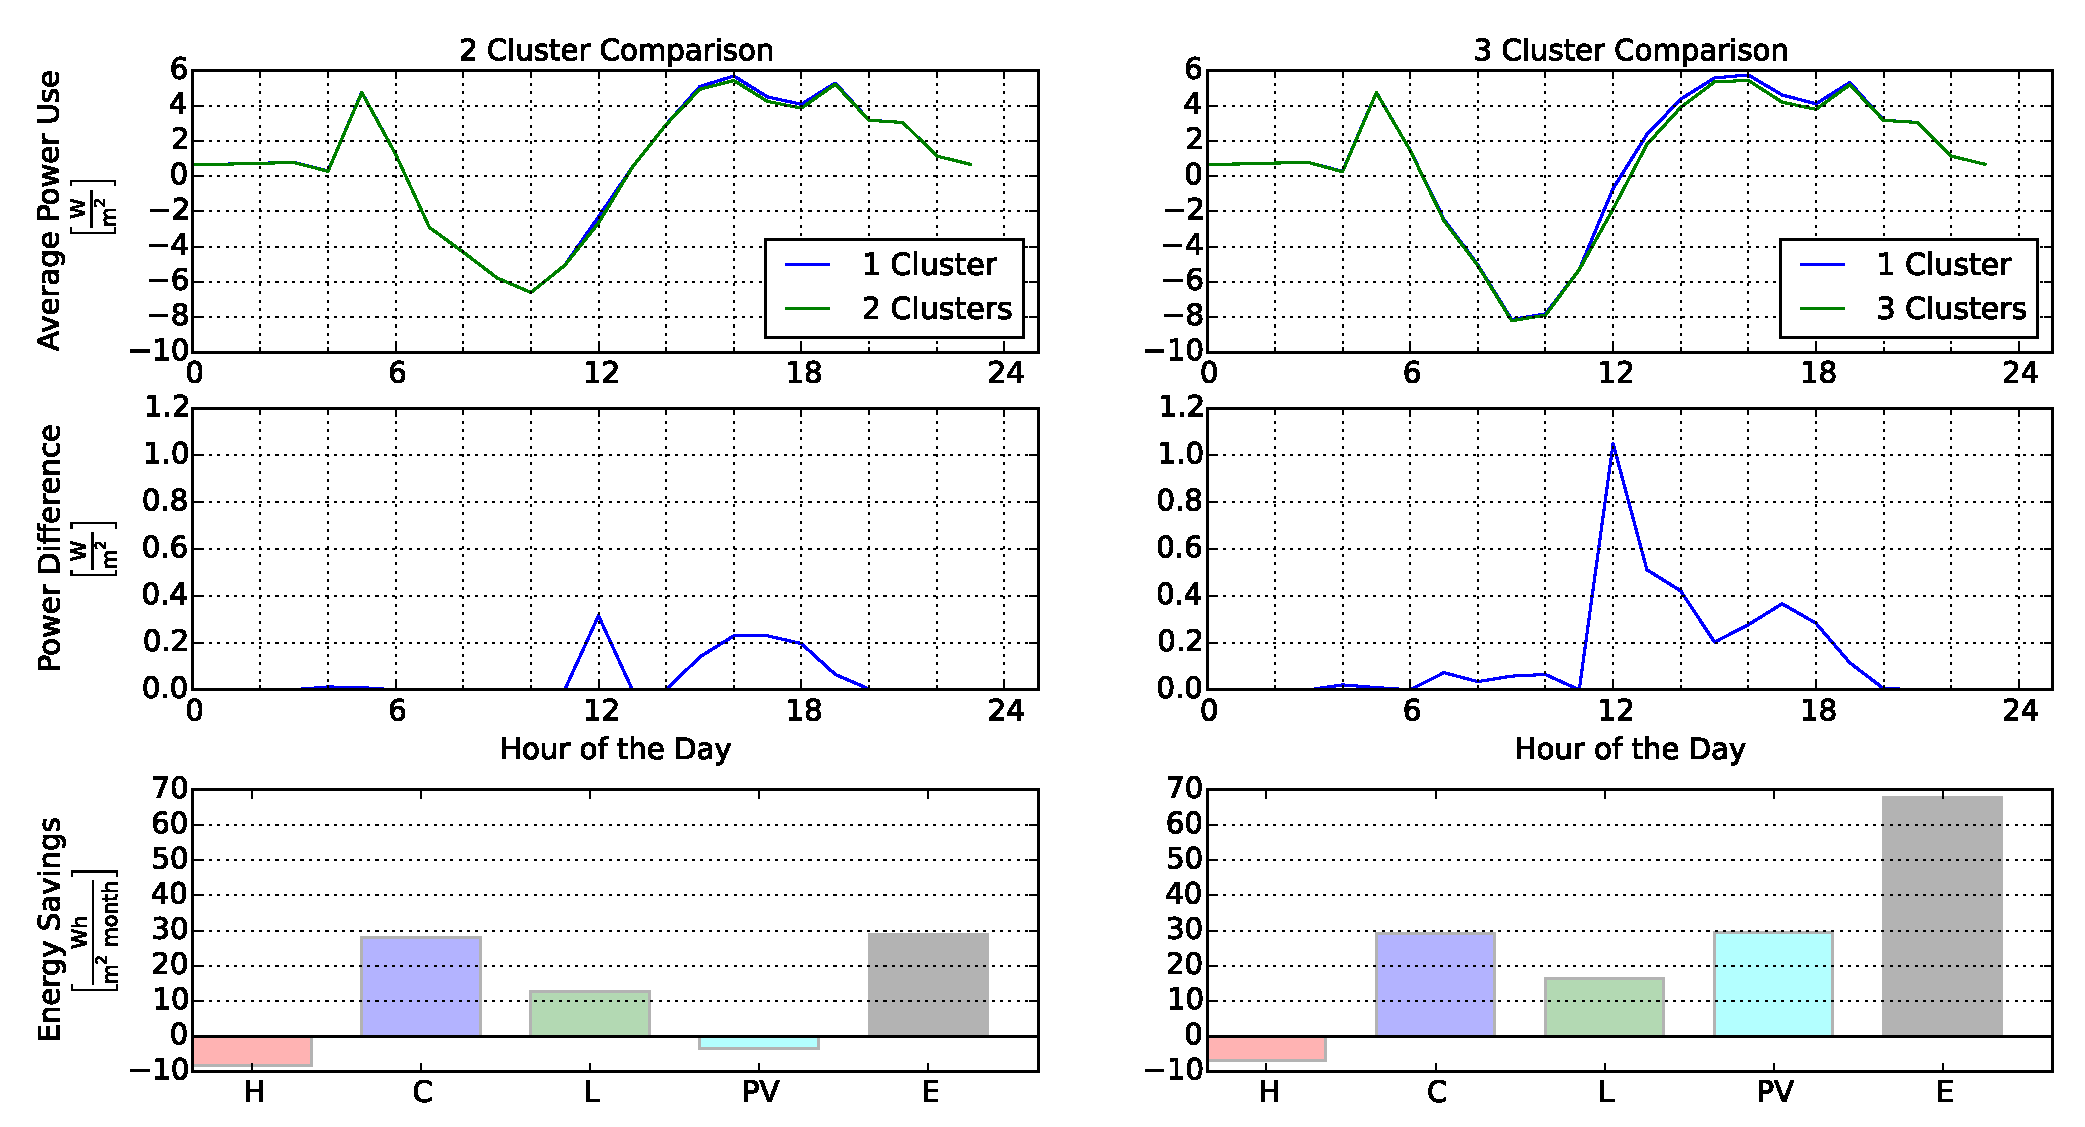
\includegraphics[width=\textwidth, trim= 0cm 0cm 0cm 0cm,clip]{cluster}
		\caption{Cluster analysis of the ASF}
		\label{fig:cluster}
		\end{center}
	\end{figure*}